%% Supplementary material: everything that supports the paper but does not fit its 12-15 pages.
%% Tables and figures are generated by scripts/build_paper.py. Numbered S1, S2, ... so the paper can cite them.
\documentclass[a4paper,11pt]{article}
\usepackage[margin=2cm]{geometry}
\usepackage{booktabs,graphicx,rotating,amsmath,amssymb,algorithm,algpseudocode}
\usepackage[hidelinks]{hyperref}

\newcommand{\ours}{DR-IMOEA}   % keep in sync with main.tex
\renewcommand{\thetable}{S\arabic{table}}
\renewcommand{\thefigure}{S\arabic{figure}}
\renewcommand{\thealgorithm}{S\arabic{algorithm}}
\renewcommand{\thesection}{S\arabic{section}}

\title{Supplementary material for ``Interval multi-objective offloading of DAG workflows in uncertain
cloud--edge--end environments via decomposition-ranked three-tier environmental selection''}
\date{}

\begin{document}
\maketitle

\section{Parameters}
% generated by scripts/build_paper.py; do not edit by hand
\begin{table}[!htbp]
\centering
\footnotesize
\caption{Parameters. $^{\dagger}$ Not given by Jin et al.; our choice. Every baseline uses the same encoding, operators, evaluator, population size and number of evaluations.}
\label{tab:params}
\setlength{\tabcolsep}{3pt}
\begin{tabular}{p{0.32\linewidth}p{0.62\linewidth}}
\toprule
Parameter & Value \\
\midrule
\multicolumn{2}{l}{\textit{Environment (Jin et al.'s Table~1; Suite B uses their small scale)}} \\
\quad Mobile-device CPU frequency & $[0.45, 0.59]$, $[0.54, 0.71]$, $[0.63, 0.82]$, $[0.72, 0.94]$, $[0.81, 1.06]$, $[0.9, 1.18]$ GHz, cycled over devices \\
\quad Device energy per Gcycle$^{\dagger}$ & $[0.9, 1.1]$ J \\
\quad Transmit / idle power & \{0.1, 0.2, 0.4, 0.5\} W / 0.02 W \\
\quad Edge-server CPU (shared by its tasks) & $[78.5, 90]$, $[102, 120]$, $[127.5, 150]$ GHz \\
\quad Cloud CPU per task & $[18, 22]$ GHz \\
\quad Wireless bandwidth / channel gain / noise & $[9, 12]$ MHz / 0.001 / $-100$ dBm \\
\quad Edge--cloud link & $[408, 624]$ Mbps \\
\quad Edge--edge link$^{\dagger}$ / downlink$^{\dagger}$ & $[408, 624]$ Mbps / equal to the uplink \\
\quad Prices $\eta_E$ / $\eta_C$ & 0.001 \$/(GHz s) / 0.01 \$/s \\
\quad Task workload / data per DAG edge & 1--5 Gcycles / 500--3000 KB, data $\times$1, $\times$20, $\times$100 \\
\quad Suite A (edge servers, tasks, devices) & small-20: 3, 100, 20; small-50: 3, 100, 50; basic-60: 6, 300, 60; basic-100: 6, 300, 100; medium-100: 10, 500, 100; medium-250: 10, 500, 250 \\
\quad Suite B & 3 edge servers, 6 devices (one origin), 5 workflow families, 100 / 400 / 1000 / 2000 tasks \\
\midrule
\multicolumn{2}{l}{\textit{\ours{}}} \\
\quad Population size $N$ / generations $G$ & 105 / 1000 (105,105 evaluations per run) \\
\quad Selection weights $(\alpha, \beta, \gamma)$ & $(5/6, 1/6, 0)$: 88 places by Rank C, 17 by Rank D, 0 by Rank U \\
\quad Rank C & interval Tchebycheff, 105 Das--Dennis weight vectors ($q = 13$), objectives normalised over the pool \\
\quad Rank C tie-break & descending interval crowding distance \\
\quad Interval crowding neighbours $k$ & $\mathrm{round}(\sqrt{2N}) = 14$ \\
\quad Interval dominance threshold & possibility degree 0.5 \\
\quad Mating & partner among the $T = 10$ nearest (normalised midpoints) with probability 1 \\
\quad Crossover & DAEC on the allocation string (gene from either parent with probability 0.5), POX on the priority string; $p_c = 0.7$ / $0.9$ (top / bottom half by uncertainty front) \\
\quad Mutation & reassign each task with probability $1/K$; shift each task within its precedence window with probability $1/K$ \\
\quad Clone removal & yes (identical genotypes skipped in selection) \\
\midrule
\multicolumn{2}{l}{\textit{Protocol}} \\
\quad Runs & 30 for \ours{}, IMOEA/D and the Jin backbone; 10 for the others; paired seeds \\
\quad Metrics & IGD on midpoints (pooled reference front), HV (mean of lower- and upper-bound HV, reference 1.1), Imprecision \\
\quad Statistics & Wilcoxon rank-sum, Holm-corrected, $\alpha = 0.05$; Friedman with Nemenyi CD \\
\quad Action set of the learned controllers & 28 Das--Dennis actions ($q = 6$) \\
\bottomrule
\end{tabular}
\end{table}


\section{Algorithms and complexity}
% Pseudocode of the method (R2). Written by hand to match the code:
%   Algorithm 1 gat_imoea_dqn/algorithm.py run() with policy "fixed" and backbone "final"
%   Algorithm 2 gat_imoea_dqn/operators.py make_offspring() with partner "neighbours"
%   Algorithm 3 gat_imoea_dqn/selection.py environmental_selection() with convergence "tchebycheff"
%   Algorithm 4 gat_imoea_dqn/evaluator.py (interval critical-path calculus)
% Needs \usepackage{algorithm,algpseudocode,amsmath} and \newcommand{\ours}{...}.

\begin{algorithm}[!htbp]
\caption{\ours{}: main loop}
\label{alg:main}
\begin{algorithmic}[1]
\Require DAG $\mathcal{G} = (V, E)$ with $K = |V|$ tasks, environment, population size $N$, generations $G_{\max}$,
  selection weights $(\alpha, \beta, \gamma)$, neighbourhood size $T$
\Ensure first interval non-dominated front of the final population
\State $W \gets$ $N$ Das--Dennis weight vectors in $\mathbb{R}^3$
\State $P \gets \emptyset$
\For{$i = 1, \dots, N$}
  \State $\mathbf{x}_i \gets$ for every task, a node drawn uniformly from those its device can reach
  \State $\mathbf{o}_i \gets$ randomised Kahn order of $\mathcal{G}$ (uniform among ready tasks)
  \State $P \gets P \cup \{(\mathbf{x}_i, \mathbf{o}_i)\}$
\EndFor
\State $\tilde{F}(P) \gets \Call{Evaluate}{P}$ \Comment{Algorithm~\ref{alg:eval}}
\For{$t = 1, \dots, G_{\max}$}
  \State $Q \gets \Call{Variation}{P, \tilde{F}(P), T}$ \Comment{Algorithm~\ref{alg:var}; $|Q| = N$}
  \State $\tilde{F}(Q) \gets \Call{Evaluate}{Q}$
  \State $P \gets \Call{Select}{P \cup Q, N, (\alpha, \beta, \gamma), W}$ \Comment{Algorithm~\ref{alg:sel}}
\EndFor
\State \Return the first front of $P$ under interval dominance
\end{algorithmic}
\end{algorithm}

\begin{algorithm}[!htbp]
\caption{\textsc{Variation}: neighbourhood mating, DAEC / POX crossover and DAG-valid mutation}
\label{alg:var}
\begin{algorithmic}[1]
\Require population $P = \{(\mathbf{x}_i, \mathbf{o}_i)\}_{i=1}^{N}$ with interval objectives $\tilde{F}_i = [F^L_i, F^U_i]$, neighbourhood size $T$
\State $\bar{F}_i \gets$ midpoint of $\tilde{F}_i$, each objective scaled to $[0, 1]$ over $P$
\State $B(i) \gets$ the $T$ members nearest to $i$ in Euclidean distance on $\bar{F}$
\State $r_{IN}(i) \gets$ index of $i$'s front under interval dominance
\State $r_{UN}(i) \gets$ index of $i$'s front under Pareto dominance on $(U_1, U_2)$ \Comment{sum and product of widths}
\State $p_c(i) \gets 0.7$ if $i$ is in the better half by $r_{UN}$, else $0.9$
\For{$i = 1, \dots, N$}
  \State $j \gets$ uniform from $B(i)$
  \State $(\mathbf{x}, \mathbf{o}) \gets (\mathbf{x}_i, \mathbf{o}_i)$
  \If{$\mathrm{rand}() < p_c(i)$}
    \State $b, w \gets$ the better and the worse of $i, j$ by $(r_{IN}, r_{UN})$
    \State $\mathbf{x} \gets$ DAEC$(\mathbf{x}_b, \mathbf{x}_w)$ \Comment{each gene from either parent with probability $1/2$}
    \State $\mathbf{o} \gets$ POX$(\mathbf{o}_i, \mathbf{o}_j)$ \Comment{precedence-preserving}
  \EndIf
  \For{each task $k$}
    \State with probability $1/K$: $x_k \gets$ another node reachable from $k$'s device
    \State with probability $1/K$: move $k$ in $\mathbf{o}$ to a random position after its last predecessor and before its first successor
  \EndFor
  \State $q_i \gets (\mathbf{x}, \mathbf{o})$ \Comment{valid by construction; no repair is needed}
\EndFor
\State \Return $Q = \{q_i\}_{i=1}^{N}$
\end{algorithmic}
\end{algorithm}

\begin{algorithm}[!htbp]
\caption{\textsc{Select}: three-tier environmental selection with a Tchebycheff Rank C}
\label{alg:sel}
\begin{algorithmic}[1]
\Require pool $M$ ($|M| = 2N$) with $\tilde{F} = [F^L, F^U]$, size $N$, weights $(\alpha, \beta, \gamma)$, weight vectors $W$
\State $n_C \gets \mathrm{round}(\alpha N)$, \; $n_D \gets \min(\mathrm{round}(\beta N), N - n_C)$, \; $n_U \gets N - n_C - n_D$
\State $G^L, G^U \gets$ $F^L, F^U$ scaled per objective by $(F - \min_M F^L) / (\max_M F^U - \min_M F^L)$
\For{each $\mathbf{w} \in W$}
  \State $g_{\mathbf{w}}(x) \gets \tfrac{1}{2}\big(\max_m w_m G^L_m(x) + \max_m w_m G^U_m(x)\big)$ for every $x \in M$
  \State $\pi_{\mathbf{w}} \gets$ $M$ sorted by ascending $g_{\mathbf{w}}$
\EndFor
\State $R_C(x) \gets \min_{\mathbf{w} \in W}$ position of $x$ in $\pi_{\mathbf{w}}$ \Comment{Rank C (replaces $R_{IN}$)}
\State $\mathrm{ICD}(x) \gets$ sum of $\mathrm{ICD}(x, y)$ over the $\mathrm{round}(\sqrt{2N})$ most similar $y$ \Comment{Rank D}
\State $R_U(x) \gets$ dominance degree of $x$ under Pareto dominance on $(U_1, U_2)$ \Comment{Rank U}
\State $L_C \gets M$ by ascending $R_C$, ties by descending ICD; \; $L_D \gets M$ by descending ICD; \; $L_U \gets M$ by ascending $R_U$
\State $S \gets \emptyset$
\For{$(L, n) \in \big((L_C, n_C), (L_D, n_D), (L_U, n_U)\big)$}
  \State append to $S$ the first $n$ members of $L$ that are not in $S$ and are not genotype copies of a member of $S$
\EndFor
\State if $|S| < N$ (only copies were left), fill $S$ from $L_C$
\State \Return $S$
\end{algorithmic}
\end{algorithm}

\begin{algorithm}[!htbp]
\caption{\textsc{Evaluate}: interval critical-path calculus for one solution $(\mathbf{x}, \mathbf{o})$}
\label{alg:eval}
\begin{algorithmic}[1]
\State $n_u \gets |\{k : x_k = u\}|$ for every edge server $u$; \; $\tilde{f}_k \gets$ $\tilde{f}_{\mathrm{dev}}$, $\tilde{f}_u / n_u$ or $\tilde{f}_C$ by the tier of $x_k$
\State $\mathrm{avail}(d) \gets [0, 0]$ for every device $d$ \Comment{a device runs one task at a time}
\For{$k$ in the order $\mathbf{o}$}
  \State $\widetilde{AT}_k \gets$ upload time of $k$'s external input if $k$ is offloaded, else $[0, 0]$
  \For{each predecessor $p$ of $k$}
    \State $\widetilde{AT}_k \gets \max\big(\widetilde{AT}_k, \widetilde{FT}_p + \tilde{D}_{pk} / \tilde{R}(x_p, x_k)\big)$ \Comment{zero transfer if co-located}
  \EndFor
  \State $\widetilde{ST}_k \gets \max(\widetilde{AT}_k, \mathrm{avail}(x_k))$ if $x_k$ is a device, else $\widetilde{AT}_k$
  \State $\widetilde{FT}_k \gets \widetilde{ST}_k + \tilde{C}_k / \tilde{f}_k$; \; if $x_k$ is a device, $\mathrm{avail}(x_k) \gets \widetilde{FT}_k$
\EndFor
\State $\tilde{F}_1 \gets \sum_{\text{applications}} \max_{k} \big(\widetilde{FT}_k + \text{return time of $k$'s external output}\big)$ \Comment{makespan}
\State $\tilde{F}_2 \gets$ device energy: local computation, transmission and idle waiting \Comment{energy}
\State $\tilde{F}_3 \gets$ edge and cloud usage charges \Comment{cost}
\State \Return $\tilde{F} = [F^L, F^U]$; every step is monotone in each bound, so $F^L$ and $F^U$ come from the lower and upper inputs
\end{algorithmic}
\end{algorithm}

% Computational complexity (R2). Derived from the code (gat_imoea_dqn/operators.py, selection.py,
% intervals.py, evaluator.py); measured times in Table~\ref{tab:timing} (scripts/build_paper.py).
\subsection{Computational complexity}
\label{sec:complexity}

Let $N$ be the population size, $M = 3$ the number of objectives, $K = |V|$ and $|E|$ the numbers of tasks
and data dependencies, and $F$ the number of interval non-dominated fronts in a population
($F \le N$, and small in practice because most of the population soon shares the first front).
One generation of \ours{} costs the following.

\begin{itemize}
\item \emph{Variation} (Algorithm~\ref{alg:var}). The interval dominance matrix of $P$ takes $O(MN^2)$ and peeling
  its fronts $O(FN^2)$; the uncertainty fronts on $(U_1, U_2)$ take the same. The neighbourhoods need all pairwise
  midpoint distances, $O(MN^2)$, and a sort of each row, $O(N^2 \log N)$. Building one child takes $O(K + |E|)$:
  DAEC and POX are linear in $K$, a shift mutation moves a task within its precedence window in $O(K)$, and with
  mutation rate $1/K$ one task moves per child in expectation. In total $O\big(N^2(M + F + \log N) + N(K + |E|)\big)$.
\item \emph{Evaluation} (Algorithm~\ref{alg:eval}). The interval critical-path calculus visits every task and every
  dependency once, $O(K + |E|)$ per solution and $O\big(N(K + |E|)\big)$ per generation.
\item \emph{Selection} (Algorithm~\ref{alg:sel}) on the pool of $2N$. The Tchebycheff values for $N$ weight vectors take
  $O(MN^2)$ and sorting the pool once per vector $O(N^2 \log N)$; the interval crowding distance needs all pairs,
  $O(MN^2)$; the uncertainty dominance degree $O(N^2)$; filling the three tiers with genotype de-duplication $O(NK)$.
  In total $O\big(N^2(M + \log N) + NK\big)$.
\end{itemize}

A generation therefore costs $O\big(N^2(M + F + \log N) + N(K + |E|)\big)$, and a run of $G_{\max}$ generations
$O\big(G_{\max}[N^2(M + F + \log N) + N(K + |E|)]\big)$ time with $O(N^2 + NK)$ memory. Jin et al.'s Rank C, the
interval dominance degree $R_{IN}$, costs $O(MN^2)$ for the dominance matrix plus $O(N^2)$ for the degrees, so the
Tchebycheff Rank C adds only the $O(N^2 \log N)$ of the per-vector sorts; neighbourhood mating adds the same order.
Neither changes the number of evaluations, which is $N(G_{\max} + 1)$ for \ours{} and every baseline.

With $N = 105$ the population terms are about $N^2(M + \log_2 2N) \approx 1.2 \times 10^5$ elementary operations per
generation, while the evaluation term $N(K + |E|)$ grows from about $3 \times 10^4$ for the 100-task Cybershake
workflow ($|E| = 192$) to $3 \times 10^5$ at 1000 tasks and $6 \times 10^5$ at 2000. The measured times
(Table~\ref{tab:timing}) show that \ours{} needs about as long as IMOEA/D and the fixed-action Jin backbone on every
instance, and that its time grows only 1.8-fold from 100 to 2000 Cybershake tasks: the evaluation loop is compiled and
has a small constant, so the population terms, which do not depend on $K$, account for most of the run time. The
learned controller of IMOEA-DQN adds a state computation and a network forward pass every generation and a training
step every 50 generations; on the same instances this costs 2--52\% more time than the fixed-action backbone, without
improving the result (see the analysis of learned control in the paper).


\section{Per-instance results}
% generated by scripts/build_paper.py; do not edit by hand
\begin{sidewaystable}[!htbp]
\centering
\tiny
\caption{Suite A: IGD ($\times 10^{-2}$) per instance, mean (standard deviation) over the runs (lower is better). 12 instances; \ours{}, IMOEA/D and the Jin backbone 30 runs, the other methods 10.}
\label{tab:suitea_igd}
\setlength{\tabcolsep}{3pt}
\begin{tabular}{lcccccccccc}
\toprule
Instance & \ours{} & IMOEA/D & AWN & IED & IP-MOEA & NSGA-II\textsubscript{m} & NSGA-II\textsubscript{i} & NSGA-III & Jin bb. & IMOEA-DQN \\
\midrule
basic-60 $\times1$ & \textbf{1.02} (0.06) & 4.35 (0.51)$^{-}$ & 3.44 (0.34)$^{-}$ & 19.90 (1.05)$^{-}$ & 21.51 (2.04)$^{-}$ & 5.64 (0.78)$^{-}$ & 5.35 (0.51)$^{-}$ & 17.12 (3.77)$^{-}$ & 16.01 (2.85)$^{-}$ & 27.85 (4.80)$^{-}$ \\
basic-60 $\times20$ & \textbf{1.21} (0.07) & 3.54 (0.27)$^{-}$ & 3.11 (0.29)$^{-}$ & 14.09 (1.10)$^{-}$ & 15.42 (1.50)$^{-}$ & 5.69 (0.30)$^{-}$ & 5.48 (0.46)$^{-}$ & 15.95 (4.40)$^{-}$ & 13.25 (2.27)$^{-}$ & 22.23 (3.35)$^{-}$ \\
basic-100 $\times1$ & \textbf{1.02} (0.07) & 3.62 (0.45)$^{-}$ & 2.75 (0.29)$^{-}$ & 17.40 (0.85)$^{-}$ & 17.16 (0.93)$^{-}$ & 4.76 (0.45)$^{-}$ & 4.62 (0.36)$^{-}$ & 12.44 (3.57)$^{-}$ & 12.39 (2.73)$^{-}$ & 31.31 (9.29)$^{-}$ \\
basic-100 $\times20$ & \textbf{1.16} (0.06) & 3.15 (0.28)$^{-}$ & 2.90 (0.22)$^{-}$ & 12.82 (1.32)$^{-}$ & 14.21 (1.02)$^{-}$ & 4.88 (0.32)$^{-}$ & 4.87 (0.20)$^{-}$ & 17.84 (6.37)$^{-}$ & 13.35 (2.27)$^{-}$ & 28.54 (10.52)$^{-}$ \\
medium-100 $\times1$ & \textbf{1.02} (0.08) & 3.06 (0.29)$^{-}$ & 3.07 (1.06)$^{-}$ & 14.74 (0.48)$^{-}$ & 20.23 (1.55)$^{-}$ & 6.44 (0.57)$^{-}$ & 6.31 (0.40)$^{-}$ & 16.06 (4.93)$^{-}$ & 15.50 (2.18)$^{-}$ & 33.51 (7.61)$^{-}$ \\
medium-100 $\times20$ & \textbf{1.19} (0.08) & 2.99 (0.30)$^{-}$ & 3.63 (0.85)$^{-}$ & 12.00 (0.56)$^{-}$ & 17.35 (1.81)$^{-}$ & 6.66 (0.13)$^{-}$ & 6.56 (0.48)$^{-}$ & 21.50 (6.15)$^{-}$ & 15.62 (2.88)$^{-}$ & 32.45 (10.81)$^{-}$ \\
medium-250 $\times1$ & \textbf{1.17} (0.09) & 2.80 (0.25)$^{-}$ & 2.97 (0.60)$^{-}$ & 13.04 (0.82)$^{-}$ & 19.27 (1.89)$^{-}$ & 5.97 (0.58)$^{-}$ & 6.01 (0.45)$^{-}$ & 14.23 (1.85)$^{-}$ & 15.23 (1.95)$^{-}$ & 38.28 (8.79)$^{-}$ \\
medium-250 $\times20$ & \textbf{1.14} (0.09) & 3.43 (0.35)$^{-}$ & 4.03 (1.01)$^{-}$ & 15.31 (4.65)$^{-}$ & 17.81 (1.15)$^{-}$ & 6.89 (0.38)$^{-}$ & 6.89 (0.47)$^{-}$ & 23.40 (2.11)$^{-}$ & 16.20 (1.82)$^{-}$ & 29.04 (8.55)$^{-}$ \\
small-20 $\times1$ & \textbf{1.28} (0.05) & 3.50 (0.52)$^{-}$ & 2.65 (0.47)$^{-}$ & 10.96 (1.41)$^{-}$ & 10.20 (1.77)$^{-}$ & 2.55 (0.15)$^{-}$ & 2.88 (0.21)$^{-}$ & 6.35 (4.63)$^{-}$ & 5.50 (1.52)$^{-}$ & 10.28 (3.34)$^{-}$ \\
small-20 $\times20$ & \textbf{1.61} (0.08) & 2.99 (0.31)$^{-}$ & 2.33 (0.34)$^{-}$ & 8.59 (3.14)$^{-}$ & 8.87 (1.64)$^{-}$ & 3.24 (0.21)$^{-}$ & 3.27 (0.29)$^{-}$ & 6.74 (2.40)$^{-}$ & 6.04 (0.81)$^{-}$ & 19.15 (13.11)$^{-}$ \\
small-50 $\times1$ & \textbf{1.43} (0.06) & 2.38 (0.36)$^{-}$ & 1.85 (0.16)$^{-}$ & 5.81 (2.70)$^{-}$ & 6.79 (1.32)$^{-}$ & 2.40 (0.19)$^{-}$ & 2.45 (0.20)$^{-}$ & 4.31 (1.42)$^{-}$ & 4.76 (0.50)$^{-}$ & 19.64 (13.27)$^{-}$ \\
small-50 $\times20$ & \textbf{1.41} (0.09) & 2.47 (0.29)$^{-}$ & 2.15 (0.34)$^{-}$ & 4.09 (0.28)$^{-}$ & 7.72 (1.30)$^{-}$ & 2.90 (0.25)$^{-}$ & 2.86 (0.31)$^{-}$ & 7.41 (2.24)$^{-}$ & 6.05 (0.86)$^{-}$ & 12.89 (6.28)$^{-}$ \\
\midrule
$+/-/\approx$ & -- & 0/12/0 & 0/12/0 & 0/12/0 & 0/12/0 & 0/12/0 & 0/12/0 & 0/12/0 & 0/12/0 & 0/12/0 \\
\bottomrule
\end{tabular}
\par\smallskip
\parbox{\linewidth}{\footnotesize $^{+}$ / $^{-}$ / $^{\approx}$: significantly better / worse than \ours{} / no significant difference (Wilcoxon rank-sum, two-sided, Holm-corrected over the compared methods, $\alpha = 0.05$). Best mean per row in bold.}
\end{sidewaystable}

% generated by scripts/build_paper.py; do not edit by hand
\begin{sidewaystable}[!htbp]
\centering
\tiny
\caption{Suite A: HV per instance, mean (standard deviation) over the runs (higher is better). 12 instances; \ours{}, IMOEA/D and the Jin backbone 30 runs, the other methods 10.}
\label{tab:suitea_hv_jin}
\setlength{\tabcolsep}{3pt}
\begin{tabular}{lcccccccccc}
\toprule
Instance & \ours{} & IMOEA/D & AWN & IED & IP-MOEA & NSGA-II\textsubscript{m} & NSGA-II\textsubscript{i} & NSGA-III & Jin bb. & IMOEA-DQN \\
\midrule
basic-60 $\times1$ & \textbf{0.771} (0.002) & 0.740 (0.004)$^{-}$ & 0.746 (0.003)$^{-}$ & 0.611 (0.007)$^{-}$ & 0.581 (0.010)$^{-}$ & 0.721 (0.005)$^{-}$ & 0.725 (0.006)$^{-}$ & 0.628 (0.028)$^{-}$ & 0.575 (0.028)$^{-}$ & 0.541 (0.038)$^{-}$ \\
basic-60 $\times20$ & \textbf{0.793} (0.002) & 0.765 (0.003)$^{-}$ & 0.767 (0.003)$^{-}$ & 0.640 (0.009)$^{-}$ & 0.603 (0.011)$^{-}$ & 0.735 (0.004)$^{-}$ & 0.738 (0.005)$^{-}$ & 0.624 (0.032)$^{-}$ & 0.576 (0.032)$^{-}$ & 0.567 (0.026)$^{-}$ \\
basic-100 $\times1$ & \textbf{0.766} (0.002) & 0.741 (0.004)$^{-}$ & 0.747 (0.003)$^{-}$ & 0.615 (0.006)$^{-}$ & 0.592 (0.010)$^{-}$ & 0.723 (0.004)$^{-}$ & 0.726 (0.003)$^{-}$ & 0.647 (0.026)$^{-}$ & 0.582 (0.029)$^{-}$ & 0.510 (0.060)$^{-}$ \\
basic-100 $\times20$ & \textbf{0.823} (0.002) & 0.795 (0.003)$^{-}$ & 0.796 (0.003)$^{-}$ & 0.665 (0.021)$^{-}$ & 0.637 (0.011)$^{-}$ & 0.767 (0.004)$^{-}$ & 0.767 (0.004)$^{-}$ & 0.640 (0.049)$^{-}$ & 0.598 (0.029)$^{-}$ & 0.560 (0.072)$^{-}$ \\
medium-100 $\times1$ & \textbf{0.785} (0.003) & 0.768 (0.003)$^{-}$ & 0.763 (0.008)$^{-}$ & 0.660 (0.004)$^{-}$ & 0.592 (0.017)$^{-}$ & 0.714 (0.006)$^{-}$ & 0.715 (0.004)$^{-}$ & 0.632 (0.030)$^{-}$ & 0.549 (0.027)$^{-}$ & 0.550 (0.043)$^{-}$ \\
medium-100 $\times20$ & \textbf{0.798} (0.003) & 0.779 (0.004)$^{-}$ & 0.766 (0.009)$^{-}$ & 0.619 (0.015)$^{-}$ & 0.594 (0.013)$^{-}$ & 0.713 (0.006)$^{-}$ & 0.715 (0.010)$^{-}$ & 0.602 (0.032)$^{-}$ & 0.547 (0.025)$^{-}$ & 0.536 (0.058)$^{-}$ \\
medium-250 $\times1$ & \textbf{0.782} (0.004) & 0.769 (0.002)$^{-}$ & 0.764 (0.006)$^{-}$ & 0.665 (0.005)$^{-}$ & 0.589 (0.007)$^{-}$ & 0.716 (0.006)$^{-}$ & 0.717 (0.006)$^{-}$ & 0.639 (0.012)$^{-}$ & 0.543 (0.021)$^{-}$ & 0.513 (0.038)$^{-}$ \\
medium-250 $\times20$ & \textbf{0.847} (0.003) & 0.820 (0.004)$^{-}$ & 0.810 (0.010)$^{-}$ & 0.635 (0.022)$^{-}$ & 0.655 (0.008)$^{-}$ & 0.760 (0.008)$^{-}$ & 0.761 (0.005)$^{-}$ & 0.647 (0.010)$^{-}$ & 0.594 (0.029)$^{-}$ & 0.605 (0.048)$^{-}$ \\
small-20 $\times1$ & \textbf{0.891} (0.002) & 0.871 (0.004)$^{-}$ & 0.876 (0.003)$^{-}$ & 0.806 (0.010)$^{-}$ & 0.784 (0.017)$^{-}$ & 0.880 (0.001)$^{-}$ & 0.878 (0.002)$^{-}$ & 0.844 (0.034)$^{-}$ & 0.794 (0.025)$^{-}$ & 0.799 (0.032)$^{-}$ \\
small-20 $\times20$ & \textbf{0.865} (0.002) & 0.844 (0.003)$^{-}$ & 0.852 (0.004)$^{-}$ & 0.782 (0.032)$^{-}$ & 0.758 (0.014)$^{-}$ & 0.843 (0.002)$^{-}$ & 0.843 (0.002)$^{-}$ & 0.799 (0.025)$^{-}$ & 0.760 (0.020)$^{-}$ & 0.690 (0.089)$^{-}$ \\
small-50 $\times1$ & \textbf{0.819} (0.002) & 0.803 (0.004)$^{-}$ & 0.805 (0.002)$^{-}$ & 0.763 (0.029)$^{-}$ & 0.727 (0.018)$^{-}$ & 0.808 (0.001)$^{-}$ & 0.808 (0.002)$^{-}$ & 0.777 (0.017)$^{-}$ & 0.727 (0.014)$^{-}$ & 0.645 (0.092)$^{-}$ \\
small-50 $\times20$ & \textbf{0.887} (0.001) & 0.867 (0.004)$^{-}$ & 0.871 (0.004)$^{-}$ & 0.835 (0.004)$^{-}$ & 0.780 (0.016)$^{-}$ & 0.861 (0.003)$^{-}$ & 0.861 (0.003)$^{-}$ & 0.801 (0.025)$^{-}$ & 0.774 (0.024)$^{-}$ & 0.736 (0.049)$^{-}$ \\
\midrule
$+/-/\approx$ & -- & 0/12/0 & 0/12/0 & 0/12/0 & 0/12/0 & 0/12/0 & 0/12/0 & 0/12/0 & 0/12/0 & 0/12/0 \\
\bottomrule
\end{tabular}
\par\smallskip
\parbox{\linewidth}{\footnotesize $^{+}$ / $^{-}$ / $^{\approx}$: significantly better / worse than \ours{} / no significant difference (Wilcoxon rank-sum, two-sided, Holm-corrected over the compared methods, $\alpha = 0.05$). Best mean per row in bold.}
\end{sidewaystable}

% generated by scripts/build_paper.py; do not edit by hand
\begin{sidewaystable}[!htbp]
\centering
\tiny
\caption{Suite B: IGD ($\times 10^{-2}$) per instance, mean (standard deviation) over the runs (lower is better). 45 instances; \ours{}, IMOEA/D and the Jin backbone 30 runs, the other methods 10.}
\label{tab:suiteb_igd}
\setlength{\tabcolsep}{3pt}
\begin{tabular}{lcccccccccc}
\toprule
Instance & \ours{} & IMOEA/D & AWN & IED & IP-MOEA & NSGA-II\textsubscript{m} & NSGA-II\textsubscript{i} & NSGA-III & Jin bb. & IMOEA-DQN \\
\midrule
cybershake-100 $\times1$ & 0.74 (0.08) & 1.45 (0.21)$^{-}$ & 0.95 (0.08)$^{-}$ & 4.21 (0.61)$^{-}$ & 2.96 (0.62)$^{-}$ & \textbf{0.59} (0.05)$^{+}$ & 0.59 (0.03)$^{+}$ & 3.28 (3.17)$^{-}$ & 2.93 (0.48)$^{-}$ & 20.75 (13.02)$^{-}$ \\
cybershake-100 $\times20$ & \textbf{1.14} (0.06) & 1.52 (0.14)$^{-}$ & 1.26 (0.09)$^{-}$ & 3.98 (0.24)$^{-}$ & 4.33 (0.92)$^{-}$ & 1.44 (0.15)$^{-}$ & 1.47 (0.09)$^{-}$ & 3.94 (1.51)$^{-}$ & 4.37 (1.21)$^{-}$ & 16.92 (11.08)$^{-}$ \\
cybershake-100 $\times100$ & \textbf{2.06} (0.20) & 2.40 (0.25)$^{-}$ & 2.26 (0.28)$^{-}$ & 4.43 (0.48)$^{-}$ & 6.44 (1.04)$^{-}$ & 3.03 (0.29)$^{-}$ & 2.79 (0.35)$^{-}$ & 6.21 (8.44)$^{-}$ & 5.94 (0.90)$^{-}$ & 14.90 (7.89)$^{-}$ \\
cybershake-400 $\times1$ & \textbf{0.65} (0.05) & 0.89 (0.11)$^{-}$ & 1.18 (0.12)$^{-}$ & 14.39 (3.18)$^{-}$ & 9.39 (0.95)$^{-}$ & 3.34 (0.69)$^{-}$ & 3.97 (0.77)$^{-}$ & 10.74 (3.03)$^{-}$ & 9.93 (1.66)$^{-}$ & 19.45 (4.15)$^{-}$ \\
cybershake-400 $\times20$ & \textbf{1.27} (0.11) & 1.58 (0.13)$^{-}$ & 1.99 (0.21)$^{-}$ & 13.44 (3.84)$^{-}$ & 11.64 (0.77)$^{-}$ & 4.99 (0.50)$^{-}$ & 4.60 (0.94)$^{-}$ & 11.98 (0.96)$^{-}$ & 9.40 (1.18)$^{-}$ & 21.77 (4.04)$^{-}$ \\
cybershake-400 $\times100$ & \textbf{2.61} (0.39) & 3.40 (0.81)$^{-}$ & 4.14 (0.90)$^{-}$ & 15.44 (1.72)$^{-}$ & 15.41 (1.31)$^{-}$ & 6.80 (0.70)$^{-}$ & 7.32 (0.61)$^{-}$ & 16.19 (3.27)$^{-}$ & 11.14 (1.65)$^{-}$ & 27.89 (10.37)$^{-}$ \\
cybershake-1000 $\times1$ & \textbf{2.76} (0.33) & 3.01 (0.33)$^{-}$ & 9.14 (0.63)$^{-}$ & 21.79 (0.99)$^{-}$ & 17.10 (1.16)$^{-}$ & 13.43 (1.14)$^{-}$ & 12.89 (1.16)$^{-}$ & 20.06 (0.89)$^{-}$ & 17.46 (1.39)$^{-}$ & 27.15 (2.57)$^{-}$ \\
cybershake-1000 $\times20$ & \textbf{2.76} (0.35) & 3.21 (0.22)$^{-}$ & 8.38 (0.63)$^{-}$ & 18.59 (0.63)$^{-}$ & 17.39 (0.76)$^{-}$ & 12.16 (0.78)$^{-}$ & 11.79 (1.04)$^{-}$ & 18.30 (1.20)$^{-}$ & 15.86 (1.24)$^{-}$ & 28.52 (4.70)$^{-}$ \\
cybershake-1000 $\times100$ & \textbf{3.47} (0.57) & 5.41 (0.37)$^{-}$ & 8.90 (0.62)$^{-}$ & 20.76 (1.95)$^{-}$ & 21.38 (0.84)$^{-}$ & 13.93 (0.85)$^{-}$ & 14.28 (0.95)$^{-}$ & 24.69 (1.44)$^{-}$ & 16.88 (1.34)$^{-}$ & 32.75 (3.80)$^{-}$ \\
epigenomics-100 $\times1$ & 0.81 (0.09) & 1.79 (0.23)$^{-}$ & 1.15 (0.19)$^{-}$ & 5.39 (1.17)$^{-}$ & 5.00 (1.31)$^{-}$ & 0.74 (0.17)$^{\approx}$ & \textbf{0.68} (0.10)$^{+}$ & 8.34 (6.69)$^{-}$ & 4.36 (1.15)$^{-}$ & 25.50 (11.27)$^{-}$ \\
epigenomics-100 $\times20$ & \textbf{1.07} (0.07) & 2.00 (0.18)$^{-}$ & 1.57 (0.19)$^{-}$ & 5.68 (0.35)$^{-}$ & 6.71 (1.06)$^{-}$ & 1.79 (0.21)$^{-}$ & 1.84 (0.20)$^{-}$ & 5.19 (1.83)$^{-}$ & 5.83 (1.43)$^{-}$ & 23.88 (10.74)$^{-}$ \\
epigenomics-100 $\times100$ & \textbf{1.75} (0.10) & 2.04 (0.43)$^{-}$ & 2.11 (0.38)$^{-}$ & 6.18 (0.86)$^{-}$ & 6.63 (0.70)$^{-}$ & 4.96 (0.56)$^{-}$ & 5.23 (0.97)$^{-}$ & 9.41 (4.80)$^{-}$ & 8.36 (1.62)$^{-}$ & 15.10 (10.02)$^{-}$ \\
epigenomics-400 $\times1$ & \textbf{0.61} (0.09) & 0.84 (0.09)$^{-}$ & 1.12 (0.14)$^{-}$ & 14.28 (4.15)$^{-}$ & 9.89 (0.85)$^{-}$ & 4.24 (0.40)$^{-}$ & 4.21 (0.57)$^{-}$ & 11.40 (1.92)$^{-}$ & 10.87 (1.95)$^{-}$ & 19.48 (4.04)$^{-}$ \\
epigenomics-400 $\times20$ & \textbf{1.11} (0.08) & 1.43 (0.13)$^{-}$ & 1.68 (0.19)$^{-}$ & 24.09 (5.48)$^{-}$ & 16.81 (1.38)$^{-}$ & 6.67 (0.65)$^{-}$ & 6.62 (1.24)$^{-}$ & 20.90 (6.55)$^{-}$ & 16.83 (2.41)$^{-}$ & 27.38 (5.62)$^{-}$ \\
epigenomics-400 $\times100$ & \textbf{2.58} (0.26) & 3.51 (0.26)$^{-}$ & 4.62 (0.41)$^{-}$ & 23.46 (2.55)$^{-}$ & 21.14 (1.62)$^{-}$ & 9.40 (0.95)$^{-}$ & 10.06 (0.86)$^{-}$ & 23.30 (3.05)$^{-}$ & 19.29 (2.48)$^{-}$ & 32.12 (6.26)$^{-}$ \\
epigenomics-1000 $\times1$ & \textbf{2.58} (0.34) & 3.35 (0.37)$^{-}$ & 10.96 (0.66)$^{-}$ & 20.47 (0.73)$^{-}$ & 17.39 (0.67)$^{-}$ & 13.23 (0.32)$^{-}$ & 13.84 (0.69)$^{-}$ & 19.76 (0.69)$^{-}$ & 17.30 (1.08)$^{-}$ & 26.62 (2.57)$^{-}$ \\
epigenomics-1000 $\times20$ & \textbf{3.00} (0.31) & 3.83 (0.37)$^{-}$ & 10.16 (0.42)$^{-}$ & 19.24 (0.79)$^{-}$ & 16.33 (0.62)$^{-}$ & 12.58 (0.75)$^{-}$ & 12.61 (1.11)$^{-}$ & 18.99 (0.79)$^{-}$ & 16.78 (1.46)$^{-}$ & 27.35 (2.66)$^{-}$ \\
epigenomics-1000 $\times100$ & \textbf{4.16} (0.58) & 6.24 (0.62)$^{-}$ & 9.45 (0.89)$^{-}$ & 25.66 (1.36)$^{-}$ & 24.23 (1.37)$^{-}$ & 16.27 (0.85)$^{-}$ & 16.62 (0.79)$^{-}$ & 28.82 (1.31)$^{-}$ & 23.32 (2.38)$^{-}$ & 37.25 (4.21)$^{-}$ \\
inspiral-100 $\times1$ & 0.77 (0.06) & 1.43 (0.21)$^{-}$ & 1.01 (0.09)$^{-}$ & 4.50 (0.96)$^{-}$ & 3.64 (1.02)$^{-}$ & 0.53 (0.05)$^{+}$ & \textbf{0.53} (0.05)$^{+}$ & 3.50 (4.54)$^{-}$ & 3.16 (0.69)$^{-}$ & 15.27 (7.72)$^{-}$ \\
inspiral-100 $\times20$ & \textbf{0.90} (0.05) & 1.37 (0.14)$^{-}$ & 1.15 (0.08)$^{-}$ & 7.08 (0.91)$^{-}$ & 7.14 (0.75)$^{-}$ & 1.09 (0.06)$^{-}$ & 1.11 (0.11)$^{-}$ & 16.85 (10.47)$^{-}$ & 4.05 (0.68)$^{-}$ & 16.50 (12.59)$^{-}$ \\
inspiral-100 $\times100$ & \textbf{2.11} (0.16) & 2.21 (0.13)$^{-}$ & 2.14 (0.10)$^{\approx}$ & 4.71 (0.32)$^{-}$ & 8.26 (1.40)$^{-}$ & 3.24 (0.31)$^{-}$ & 3.07 (0.26)$^{-}$ & 11.81 (7.38)$^{-}$ & 5.69 (0.89)$^{-}$ & 14.41 (5.79)$^{-}$ \\
inspiral-400 $\times1$ & \textbf{0.53} (0.03) & 0.74 (0.11)$^{-}$ & 1.03 (0.15)$^{-}$ & 12.01 (3.98)$^{-}$ & 6.82 (0.73)$^{-}$ & 2.72 (0.41)$^{-}$ & 2.37 (0.29)$^{-}$ & 7.82 (1.15)$^{-}$ & 7.83 (1.60)$^{-}$ & 17.28 (5.46)$^{-}$ \\
inspiral-400 $\times20$ & \textbf{0.68} (0.03) & 1.05 (0.09)$^{-}$ & 1.32 (0.14)$^{-}$ & 14.57 (3.96)$^{-}$ & 13.67 (2.37)$^{-}$ & 4.26 (0.61)$^{-}$ & 4.44 (0.82)$^{-}$ & 15.90 (5.16)$^{-}$ & 11.75 (1.83)$^{-}$ & 27.43 (5.01)$^{-}$ \\
inspiral-400 $\times100$ & \textbf{2.05} (0.12) & 2.47 (0.23)$^{-}$ & 3.87 (0.29)$^{-}$ & 12.08 (1.64)$^{-}$ & 15.78 (1.61)$^{-}$ & 5.67 (0.46)$^{-}$ & 5.70 (0.41)$^{-}$ & 20.76 (2.48)$^{-}$ & 16.71 (2.52)$^{-}$ & 23.26 (4.60)$^{-}$ \\
inspiral-1000 $\times1$ & \textbf{2.55} (0.40) & 2.98 (0.30)$^{-}$ & 9.08 (0.75)$^{-}$ & 21.74 (1.07)$^{-}$ & 18.33 (1.10)$^{-}$ & 12.42 (0.88)$^{-}$ & 12.57 (1.02)$^{-}$ & 20.62 (1.12)$^{-}$ & 17.17 (1.49)$^{-}$ & 28.56 (2.56)$^{-}$ \\
inspiral-1000 $\times20$ & \textbf{3.28} (0.40) & 3.88 (0.26)$^{-}$ & 8.48 (0.63)$^{-}$ & 21.32 (0.53)$^{-}$ & 18.61 (0.51)$^{-}$ & 14.88 (0.86)$^{-}$ & 14.44 (1.11)$^{-}$ & 21.82 (1.01)$^{-}$ & 19.24 (1.18)$^{-}$ & 28.67 (2.43)$^{-}$ \\
inspiral-1000 $\times100$ & 4.97 (0.61) & \textbf{4.35} (0.44)$^{+}$ & 5.37 (0.21)$^{-}$ & 22.12 (1.03)$^{-}$ & 23.16 (1.26)$^{-}$ & 15.91 (1.26)$^{-}$ & 16.06 (1.25)$^{-}$ & 28.58 (0.62)$^{-}$ & 26.00 (1.95)$^{-}$ & 32.97 (2.63)$^{-}$ \\
montage-100 $\times1$ & 0.73 (0.06) & 1.49 (0.22)$^{-}$ & 1.01 (0.12)$^{-}$ & 4.78 (1.01)$^{-}$ & 5.45 (1.35)$^{-}$ & 0.61 (0.09)$^{+}$ & \textbf{0.60} (0.05)$^{+}$ & 9.05 (8.44)$^{-}$ & 4.07 (1.36)$^{-}$ & 17.04 (6.73)$^{-}$ \\
montage-100 $\times20$ & \textbf{1.20} (0.07) & 1.68 (0.15)$^{-}$ & 1.34 (0.10)$^{-}$ & 5.04 (0.48)$^{-}$ & 10.69 (2.26)$^{-}$ & 1.46 (0.12)$^{-}$ & 1.49 (0.19)$^{-}$ & 19.47 (8.33)$^{-}$ & 5.05 (1.46)$^{-}$ & 20.32 (11.78)$^{-}$ \\
montage-100 $\times100$ & 2.58 (0.19) & \textbf{2.54} (0.14)$^{\approx}$ & 2.55 (0.15)$^{\approx}$ & 7.36 (1.44)$^{-}$ & 11.31 (1.59)$^{-}$ & 3.42 (0.18)$^{-}$ & 3.74 (0.46)$^{-}$ & 20.58 (11.00)$^{-}$ & 7.79 (1.10)$^{-}$ & 16.69 (7.38)$^{-}$ \\
montage-400 $\times1$ & \textbf{0.58} (0.06) & 0.84 (0.13)$^{-}$ & 1.05 (0.11)$^{-}$ & 14.15 (3.74)$^{-}$ & 10.14 (0.82)$^{-}$ & 4.14 (0.34)$^{-}$ & 4.26 (0.71)$^{-}$ & 10.58 (1.37)$^{-}$ & 10.31 (1.58)$^{-}$ & 18.73 (5.70)$^{-}$ \\
montage-400 $\times20$ & \textbf{1.07} (0.06) & 1.17 (0.06)$^{-}$ & 1.35 (0.09)$^{-}$ & 20.13 (1.63)$^{-}$ & 13.14 (1.08)$^{-}$ & 4.60 (0.45)$^{-}$ & 4.80 (0.72)$^{-}$ & 15.80 (5.23)$^{-}$ & 12.66 (1.82)$^{-}$ & 20.27 (4.98)$^{-}$ \\
montage-400 $\times100$ & \textbf{2.22} (0.15) & 2.61 (0.14)$^{-}$ & 3.44 (0.32)$^{-}$ & 19.15 (1.89)$^{-}$ & 14.88 (1.20)$^{-}$ & 6.30 (0.40)$^{-}$ & 6.55 (0.37)$^{-}$ & 18.02 (2.37)$^{-}$ & 15.78 (1.54)$^{-}$ & 25.54 (6.31)$^{-}$ \\
montage-1000 $\times1$ & \textbf{1.48} (0.15) & 3.81 (0.39)$^{-}$ & 12.57 (0.54)$^{-}$ & 11.94 (0.65)$^{-}$ & 9.67 (0.56)$^{-}$ & 7.66 (0.57)$^{-}$ & 7.67 (0.34)$^{-}$ & 11.59 (0.66)$^{-}$ & 10.23 (0.88)$^{-}$ & 20.13 (3.36)$^{-}$ \\
montage-1000 $\times20$ & \textbf{2.18} (0.28) & 4.81 (0.50)$^{-}$ & 13.51 (0.76)$^{-}$ & 11.86 (0.43)$^{-}$ & 10.23 (0.34)$^{-}$ & 8.06 (0.39)$^{-}$ & 8.27 (0.44)$^{-}$ & 12.13 (1.53)$^{-}$ & 10.75 (0.87)$^{-}$ & 20.82 (3.51)$^{-}$ \\
montage-1000 $\times100$ & \textbf{4.79} (0.62) & 7.57 (0.46)$^{-}$ & 12.98 (0.69)$^{-}$ & 20.83 (0.56)$^{-}$ & 18.51 (0.94)$^{-}$ & 14.12 (0.69)$^{-}$ & 14.34 (1.03)$^{-}$ & 23.08 (0.98)$^{-}$ & 19.75 (1.61)$^{-}$ & 31.50 (2.54)$^{-}$ \\
sipht-100 $\times1$ & 0.72 (0.06) & 1.27 (0.19)$^{-}$ & 0.90 (0.07)$^{-}$ & 3.65 (0.72)$^{-}$ & 3.84 (0.90)$^{-}$ & 0.55 (0.08)$^{+}$ & \textbf{0.51} (0.05)$^{+}$ & 6.81 (8.39)$^{-}$ & 3.27 (0.46)$^{-}$ & 18.84 (11.27)$^{-}$ \\
sipht-100 $\times20$ & \textbf{0.85} (0.08) & 1.29 (0.13)$^{-}$ & 1.07 (0.12)$^{-}$ & 5.31 (0.80)$^{-}$ & 7.55 (0.73)$^{-}$ & 1.12 (0.06)$^{-}$ & 1.06 (0.16)$^{-}$ & 12.62 (4.97)$^{-}$ & 5.69 (1.88)$^{-}$ & 21.06 (9.81)$^{-}$ \\
sipht-100 $\times100$ & \textbf{1.96} (0.21) & 2.42 (0.12)$^{-}$ & 2.20 (0.10)$^{-}$ & 6.19 (1.18)$^{-}$ & 8.00 (0.89)$^{-}$ & 3.05 (0.25)$^{-}$ & 3.07 (0.26)$^{-}$ & 12.60 (5.65)$^{-}$ & 7.05 (1.22)$^{-}$ & 16.11 (5.88)$^{-}$ \\
sipht-400 $\times1$ & \textbf{0.60} (0.06) & 0.77 (0.10)$^{-}$ & 1.02 (0.13)$^{-}$ & 13.05 (4.01)$^{-}$ & 7.64 (1.00)$^{-}$ & 3.12 (0.34)$^{-}$ & 2.81 (0.35)$^{-}$ & 9.20 (1.31)$^{-}$ & 8.67 (1.21)$^{-}$ & 18.67 (4.75)$^{-}$ \\
sipht-400 $\times20$ & \textbf{0.62} (0.04) & 0.92 (0.06)$^{-}$ & 0.94 (0.10)$^{-}$ & 11.84 (1.96)$^{-}$ & 12.92 (1.41)$^{-}$ & 3.94 (0.65)$^{-}$ & 3.93 (0.79)$^{-}$ & 27.23 (5.97)$^{-}$ & 10.75 (1.74)$^{-}$ & 24.10 (6.17)$^{-}$ \\
sipht-400 $\times100$ & \textbf{1.68} (0.10) & 2.15 (0.21)$^{-}$ & 3.09 (0.19)$^{-}$ & 8.78 (1.21)$^{-}$ & 11.62 (0.84)$^{-}$ & 4.64 (0.25)$^{-}$ & 4.71 (0.31)$^{-}$ & 14.42 (3.89)$^{-}$ & 12.16 (1.67)$^{-}$ & 16.91 (3.07)$^{-}$ \\
sipht-1000 $\times1$ & \textbf{1.56} (0.17) & 3.27 (0.44)$^{-}$ & 11.31 (0.83)$^{-}$ & 15.75 (0.75)$^{-}$ & 11.80 (1.15)$^{-}$ & 8.87 (0.64)$^{-}$ & 8.99 (0.71)$^{-}$ & 15.00 (1.24)$^{-}$ & 12.36 (1.07)$^{-}$ & 22.65 (2.33)$^{-}$ \\
sipht-1000 $\times20$ & \textbf{2.48} (0.28) & 3.93 (0.36)$^{-}$ & 9.71 (0.44)$^{-}$ & 17.05 (0.56)$^{-}$ & 15.55 (0.68)$^{-}$ & 11.87 (0.76)$^{-}$ & 11.91 (0.48)$^{-}$ & 20.26 (2.53)$^{-}$ & 15.56 (0.93)$^{-}$ & 24.07 (1.53)$^{-}$ \\
sipht-1000 $\times100$ & \textbf{3.23} (0.35) & 4.73 (0.44)$^{-}$ & 5.27 (0.38)$^{-}$ & 21.87 (1.77)$^{-}$ & 22.27 (0.69)$^{-}$ & 15.13 (0.81)$^{-}$ & 15.22 (1.01)$^{-}$ & 26.09 (0.93)$^{-}$ & 23.27 (1.38)$^{-}$ & 29.91 (2.52)$^{-}$ \\
\midrule
$+/-/\approx$ & -- & 1/43/1 & 0/43/2 & 0/45/0 & 0/45/0 & 4/40/1 & 5/40/0 & 0/45/0 & 0/45/0 & 0/45/0 \\
\bottomrule
\end{tabular}
\par\smallskip
\parbox{\linewidth}{\footnotesize $^{+}$ / $^{-}$ / $^{\approx}$: significantly better / worse than \ours{} / no significant difference (Wilcoxon rank-sum, two-sided, Holm-corrected over the compared methods, $\alpha = 0.05$). Best mean per row in bold.}
\end{sidewaystable}

% generated by scripts/build_paper.py; do not edit by hand
\begin{sidewaystable}[!htbp]
\centering
\tiny
\caption{Suite B: HV per instance, mean (standard deviation) over the runs (higher is better). 45 instances; \ours{}, IMOEA/D and the Jin backbone 30 runs, the other methods 10.}
\label{tab:suiteb_hv_jin}
\setlength{\tabcolsep}{3pt}
\begin{tabular}{lcccccccccc}
\toprule
Instance & \ours{} & IMOEA/D & AWN & IED & IP-MOEA & NSGA-II\textsubscript{m} & NSGA-II\textsubscript{i} & NSGA-III & Jin bb. & IMOEA-DQN \\
\midrule
cybershake-100 $\times1$ & \textbf{0.937} (0.002) & 0.914 (0.004)$^{-}$ & 0.925 (0.002)$^{-}$ & 0.879 (0.007)$^{-}$ & 0.863 (0.011)$^{-}$ & 0.933 (0.002)$^{-}$ & 0.933 (0.002)$^{-}$ & 0.894 (0.028)$^{-}$ & 0.870 (0.013)$^{-}$ & 0.757 (0.072)$^{-}$ \\
cybershake-100 $\times20$ & \textbf{0.952} (0.002) & 0.933 (0.003)$^{-}$ & 0.942 (0.003)$^{-}$ & 0.898 (0.004)$^{-}$ & 0.857 (0.010)$^{-}$ & 0.945 (0.004)$^{-}$ & 0.945 (0.003)$^{-}$ & 0.900 (0.018)$^{-}$ & 0.867 (0.017)$^{-}$ & 0.781 (0.062)$^{-}$ \\
cybershake-100 $\times100$ & \textbf{1.024} (0.002) & 1.013 (0.003)$^{-}$ & 1.018 (0.006)$^{-}$ & 0.964 (0.010)$^{-}$ & 0.936 (0.012)$^{-}$ & 1.005 (0.003)$^{-}$ & 1.007 (0.004)$^{-}$ & 0.959 (0.057)$^{-}$ & 0.924 (0.019)$^{-}$ & 0.866 (0.048)$^{-}$ \\
cybershake-400 $\times1$ & \textbf{0.935} (0.002) & 0.923 (0.003)$^{-}$ & 0.913 (0.003)$^{-}$ & 0.788 (0.024)$^{-}$ & 0.780 (0.006)$^{-}$ & 0.886 (0.008)$^{-}$ & 0.878 (0.007)$^{-}$ & 0.814 (0.022)$^{-}$ & 0.765 (0.022)$^{-}$ & 0.741 (0.033)$^{-}$ \\
cybershake-400 $\times20$ & \textbf{0.942} (0.002) & 0.933 (0.002)$^{-}$ & 0.921 (0.005)$^{-}$ & 0.819 (0.029)$^{-}$ & 0.783 (0.009)$^{-}$ & 0.890 (0.007)$^{-}$ & 0.895 (0.008)$^{-}$ & 0.827 (0.004)$^{-}$ & 0.806 (0.014)$^{-}$ & 0.764 (0.019)$^{-}$ \\
cybershake-400 $\times100$ & \textbf{0.974} (0.003) & 0.969 (0.003)$^{-}$ & 0.961 (0.002)$^{-}$ & 0.841 (0.011)$^{-}$ & 0.826 (0.012)$^{-}$ & 0.899 (0.005)$^{-}$ & 0.895 (0.004)$^{-}$ & 0.840 (0.019)$^{-}$ & 0.825 (0.019)$^{-}$ & 0.759 (0.037)$^{-}$ \\
cybershake-1000 $\times1$ & \textbf{0.989} (0.005) & 0.982 (0.005)$^{-}$ & 0.917 (0.009)$^{-}$ & 0.865 (0.004)$^{-}$ & 0.857 (0.006)$^{-}$ & 0.888 (0.006)$^{-}$ & 0.892 (0.005)$^{-}$ & 0.874 (0.004)$^{-}$ & 0.835 (0.010)$^{-}$ & 0.770 (0.020)$^{-}$ \\
cybershake-1000 $\times20$ & \textbf{0.986} (0.006) & 0.975 (0.003)$^{-}$ & 0.911 (0.008)$^{-}$ & 0.856 (0.003)$^{-}$ & 0.851 (0.006)$^{-}$ & 0.879 (0.008)$^{-}$ & 0.878 (0.009)$^{-}$ & 0.867 (0.004)$^{-}$ & 0.815 (0.011)$^{-}$ & 0.743 (0.039)$^{-}$ \\
cybershake-1000 $\times100$ & \textbf{0.991} (0.005) & 0.973 (0.006)$^{-}$ & 0.923 (0.009)$^{-}$ & 0.821 (0.008)$^{-}$ & 0.850 (0.004)$^{-}$ & 0.842 (0.005)$^{-}$ & 0.838 (0.006)$^{-}$ & 0.837 (0.007)$^{-}$ & 0.803 (0.013)$^{-}$ & 0.699 (0.036)$^{-}$ \\
epigenomics-100 $\times1$ & \textbf{0.924} (0.002) & 0.898 (0.003)$^{-}$ & 0.909 (0.004)$^{-}$ & 0.864 (0.011)$^{-}$ & 0.838 (0.016)$^{-}$ & 0.917 (0.004)$^{-}$ & 0.918 (0.003)$^{-}$ & 0.846 (0.048)$^{-}$ & 0.847 (0.018)$^{-}$ & 0.720 (0.067)$^{-}$ \\
epigenomics-100 $\times20$ & \textbf{0.943} (0.002) & 0.920 (0.003)$^{-}$ & 0.929 (0.004)$^{-}$ & 0.882 (0.004)$^{-}$ & 0.840 (0.022)$^{-}$ & 0.923 (0.004)$^{-}$ & 0.924 (0.005)$^{-}$ & 0.887 (0.015)$^{-}$ & 0.847 (0.019)$^{-}$ & 0.753 (0.053)$^{-}$ \\
epigenomics-100 $\times100$ & \textbf{1.022} (0.002) & 1.005 (0.005)$^{-}$ & 1.006 (0.005)$^{-}$ & 0.932 (0.011)$^{-}$ & 0.889 (0.007)$^{-}$ & 0.966 (0.010)$^{-}$ & 0.970 (0.009)$^{-}$ & 0.912 (0.035)$^{-}$ & 0.861 (0.021)$^{-}$ & 0.841 (0.049)$^{-}$ \\
epigenomics-400 $\times1$ & \textbf{0.915} (0.002) & 0.903 (0.002)$^{-}$ & 0.896 (0.004)$^{-}$ & 0.760 (0.034)$^{-}$ & 0.759 (0.008)$^{-}$ & 0.850 (0.006)$^{-}$ & 0.850 (0.006)$^{-}$ & 0.782 (0.016)$^{-}$ & 0.742 (0.020)$^{-}$ & 0.710 (0.019)$^{-}$ \\
epigenomics-400 $\times20$ & \textbf{0.869} (0.004) & 0.861 (0.003)$^{-}$ & 0.857 (0.004)$^{-}$ & 0.676 (0.033)$^{-}$ & 0.711 (0.010)$^{-}$ & 0.800 (0.005)$^{-}$ & 0.801 (0.010)$^{-}$ & 0.697 (0.043)$^{-}$ & 0.691 (0.017)$^{-}$ & 0.644 (0.031)$^{-}$ \\
epigenomics-400 $\times100$ & \textbf{0.960} (0.003) & 0.942 (0.004)$^{-}$ & 0.921 (0.009)$^{-}$ & 0.785 (0.012)$^{-}$ & 0.808 (0.008)$^{-}$ & 0.859 (0.006)$^{-}$ & 0.857 (0.005)$^{-}$ & 0.796 (0.012)$^{-}$ & 0.775 (0.014)$^{-}$ & 0.733 (0.015)$^{-}$ \\
epigenomics-1000 $\times1$ & \textbf{0.996} (0.005) & 0.985 (0.005)$^{-}$ & 0.902 (0.009)$^{-}$ & 0.875 (0.004)$^{-}$ & 0.874 (0.006)$^{-}$ & 0.901 (0.005)$^{-}$ & 0.899 (0.004)$^{-}$ & 0.882 (0.004)$^{-}$ & 0.848 (0.006)$^{-}$ & 0.765 (0.031)$^{-}$ \\
epigenomics-1000 $\times20$ & \textbf{0.972} (0.005) & 0.968 (0.005)$^{-}$ & 0.897 (0.004)$^{-}$ & 0.851 (0.005)$^{-}$ & 0.850 (0.006)$^{-}$ & 0.872 (0.006)$^{-}$ & 0.870 (0.007)$^{-}$ & 0.859 (0.004)$^{-}$ & 0.815 (0.011)$^{-}$ & 0.730 (0.031)$^{-}$ \\
epigenomics-1000 $\times100$ & \textbf{0.905} (0.010) & 0.885 (0.008)$^{-}$ & 0.851 (0.010)$^{-}$ & 0.712 (0.009)$^{-}$ & 0.748 (0.005)$^{-}$ & 0.743 (0.008)$^{-}$ & 0.740 (0.009)$^{-}$ & 0.735 (0.010)$^{-}$ & 0.709 (0.010)$^{-}$ & 0.580 (0.037)$^{-}$ \\
inspiral-100 $\times1$ & \textbf{0.920} (0.002) & 0.897 (0.004)$^{-}$ & 0.907 (0.002)$^{-}$ & 0.860 (0.011)$^{-}$ & 0.848 (0.011)$^{-}$ & 0.918 (0.002)$^{\approx}$ & 0.919 (0.003)$^{\approx}$ & 0.878 (0.037)$^{-}$ & 0.847 (0.018)$^{-}$ & 0.766 (0.045)$^{-}$ \\
inspiral-100 $\times20$ & \textbf{1.002} (0.002) & 0.986 (0.003)$^{-}$ & 0.994 (0.002)$^{-}$ & 0.927 (0.008)$^{-}$ & 0.920 (0.011)$^{-}$ & 0.994 (0.002)$^{-}$ & 0.993 (0.002)$^{-}$ & 0.871 (0.062)$^{-}$ & 0.933 (0.016)$^{-}$ & 0.861 (0.065)$^{-}$ \\
inspiral-100 $\times100$ & \textbf{1.017} (0.001) & 0.997 (0.003)$^{-}$ & 1.001 (0.002)$^{-}$ & 0.946 (0.004)$^{-}$ & 0.922 (0.013)$^{-}$ & 0.987 (0.004)$^{-}$ & 0.988 (0.003)$^{-}$ & 0.897 (0.048)$^{-}$ & 0.911 (0.021)$^{-}$ & 0.860 (0.038)$^{-}$ \\
inspiral-400 $\times1$ & \textbf{0.931} (0.003) & 0.916 (0.003)$^{-}$ & 0.904 (0.006)$^{-}$ & 0.780 (0.030)$^{-}$ & 0.784 (0.007)$^{-}$ & 0.871 (0.006)$^{-}$ & 0.876 (0.006)$^{-}$ & 0.809 (0.010)$^{-}$ & 0.757 (0.021)$^{-}$ & 0.737 (0.027)$^{-}$ \\
inspiral-400 $\times20$ & \textbf{0.864} (0.003) & 0.850 (0.003)$^{-}$ & 0.845 (0.004)$^{-}$ & 0.700 (0.031)$^{-}$ & 0.695 (0.014)$^{-}$ & 0.797 (0.008)$^{-}$ & 0.795 (0.009)$^{-}$ & 0.695 (0.036)$^{-}$ & 0.685 (0.013)$^{-}$ & 0.604 (0.027)$^{-}$ \\
inspiral-400 $\times100$ & \textbf{0.980} (0.003) & 0.974 (0.003)$^{-}$ & 0.950 (0.005)$^{-}$ & 0.882 (0.021)$^{-}$ & 0.871 (0.006)$^{-}$ & 0.927 (0.005)$^{-}$ & 0.926 (0.004)$^{-}$ & 0.853 (0.011)$^{-}$ & 0.827 (0.014)$^{-}$ & 0.815 (0.015)$^{-}$ \\
inspiral-1000 $\times1$ & \textbf{0.993} (0.005) & 0.982 (0.005)$^{-}$ & 0.915 (0.008)$^{-}$ & 0.869 (0.003)$^{-}$ & 0.865 (0.003)$^{-}$ & 0.895 (0.005)$^{-}$ & 0.892 (0.008)$^{-}$ & 0.879 (0.004)$^{-}$ & 0.839 (0.009)$^{-}$ & 0.769 (0.035)$^{-}$ \\
inspiral-1000 $\times20$ & 0.954 (0.006) & \textbf{0.956} (0.003)$^{\approx}$ & 0.905 (0.007)$^{-}$ & 0.826 (0.003)$^{-}$ & 0.835 (0.004)$^{-}$ & 0.855 (0.006)$^{-}$ & 0.852 (0.006)$^{-}$ & 0.831 (0.005)$^{-}$ & 0.793 (0.009)$^{-}$ & 0.720 (0.036)$^{-}$ \\
inspiral-1000 $\times100$ & 0.833 (0.010) & \textbf{0.843} (0.005)$^{+}$ & 0.834 (0.005)$^{\approx}$ & 0.676 (0.008)$^{-}$ & 0.690 (0.008)$^{-}$ & 0.702 (0.007)$^{-}$ & 0.703 (0.010)$^{-}$ & 0.668 (0.004)$^{-}$ & 0.648 (0.006)$^{-}$ & 0.551 (0.027)$^{-}$ \\
montage-100 $\times1$ & \textbf{0.922} (0.002) & 0.897 (0.004)$^{-}$ & 0.907 (0.003)$^{-}$ & 0.861 (0.011)$^{-}$ & 0.833 (0.007)$^{-}$ & 0.916 (0.003)$^{-}$ & 0.916 (0.002)$^{-}$ & 0.835 (0.063)$^{-}$ & 0.842 (0.019)$^{-}$ & 0.762 (0.041)$^{-}$ \\
montage-100 $\times20$ & \textbf{0.941} (0.003) & 0.919 (0.003)$^{-}$ & 0.930 (0.003)$^{-}$ & 0.878 (0.005)$^{-}$ & 0.822 (0.018)$^{-}$ & 0.928 (0.003)$^{-}$ & 0.925 (0.004)$^{-}$ & 0.775 (0.052)$^{-}$ & 0.847 (0.014)$^{-}$ & 0.762 (0.067)$^{-}$ \\
montage-100 $\times100$ & \textbf{1.006} (0.003) & 0.986 (0.003)$^{-}$ & 0.992 (0.003)$^{-}$ & 0.916 (0.017)$^{-}$ & 0.873 (0.014)$^{-}$ & 0.968 (0.002)$^{-}$ & 0.965 (0.008)$^{-}$ & 0.837 (0.063)$^{-}$ & 0.860 (0.024)$^{-}$ & 0.827 (0.041)$^{-}$ \\
montage-400 $\times1$ & \textbf{0.913} (0.002) & 0.900 (0.004)$^{-}$ & 0.896 (0.005)$^{-}$ & 0.750 (0.031)$^{-}$ & 0.753 (0.008)$^{-}$ & 0.846 (0.004)$^{-}$ & 0.845 (0.009)$^{-}$ & 0.778 (0.012)$^{-}$ & 0.741 (0.019)$^{-}$ & 0.710 (0.032)$^{-}$ \\
montage-400 $\times20$ & \textbf{0.874} (0.004) & 0.863 (0.002)$^{-}$ & 0.859 (0.002)$^{-}$ & 0.660 (0.009)$^{-}$ & 0.706 (0.009)$^{-}$ & 0.802 (0.006)$^{-}$ & 0.799 (0.009)$^{-}$ & 0.694 (0.035)$^{-}$ & 0.680 (0.023)$^{-}$ & 0.648 (0.023)$^{-}$ \\
montage-400 $\times100$ & \textbf{0.941} (0.003) & 0.932 (0.003)$^{-}$ & 0.918 (0.005)$^{-}$ & 0.770 (0.005)$^{-}$ & 0.796 (0.009)$^{-}$ & 0.863 (0.006)$^{-}$ & 0.862 (0.005)$^{-}$ & 0.785 (0.012)$^{-}$ & 0.749 (0.011)$^{-}$ & 0.726 (0.025)$^{-}$ \\
montage-1000 $\times1$ & \textbf{0.998} (0.004) & 0.987 (0.004)$^{-}$ & 0.906 (0.004)$^{-}$ & 0.874 (0.004)$^{-}$ & 0.872 (0.007)$^{-}$ & 0.899 (0.006)$^{-}$ & 0.897 (0.003)$^{-}$ & 0.877 (0.004)$^{-}$ & 0.846 (0.009)$^{-}$ & 0.751 (0.046)$^{-}$ \\
montage-1000 $\times20$ & \textbf{0.999} (0.006) & 0.990 (0.005)$^{-}$ & 0.904 (0.008)$^{-}$ & 0.877 (0.002)$^{-}$ & 0.883 (0.005)$^{-}$ & 0.894 (0.006)$^{-}$ & 0.893 (0.007)$^{-}$ & 0.879 (0.007)$^{-}$ & 0.849 (0.007)$^{-}$ & 0.736 (0.048)$^{-}$ \\
montage-1000 $\times100$ & \textbf{0.948} (0.013) & 0.934 (0.004)$^{-}$ & 0.876 (0.008)$^{-}$ & 0.778 (0.008)$^{-}$ & 0.826 (0.006)$^{-}$ & 0.816 (0.007)$^{-}$ & 0.813 (0.007)$^{-}$ & 0.803 (0.008)$^{-}$ & 0.784 (0.007)$^{-}$ & 0.637 (0.039)$^{-}$ \\
sipht-100 $\times1$ & \textbf{0.955} (0.002) & 0.933 (0.004)$^{-}$ & 0.941 (0.002)$^{-}$ & 0.905 (0.008)$^{-}$ & 0.877 (0.016)$^{-}$ & 0.950 (0.004)$^{-}$ & 0.952 (0.003)$^{-}$ & 0.888 (0.060)$^{-}$ & 0.883 (0.017)$^{-}$ & 0.788 (0.063)$^{-}$ \\
sipht-100 $\times20$ & \textbf{0.968} (0.002) & 0.948 (0.003)$^{-}$ & 0.958 (0.002)$^{-}$ & 0.899 (0.007)$^{-}$ & 0.870 (0.014)$^{-}$ & 0.953 (0.002)$^{-}$ & 0.954 (0.005)$^{-}$ & 0.843 (0.038)$^{-}$ & 0.880 (0.020)$^{-}$ & 0.778 (0.061)$^{-}$ \\
sipht-100 $\times100$ & \textbf{1.041} (0.001) & 1.017 (0.003)$^{-}$ & 1.018 (0.002)$^{-}$ & 0.962 (0.009)$^{-}$ & 0.949 (0.011)$^{-}$ & 1.009 (0.004)$^{-}$ & 1.008 (0.004)$^{-}$ & 0.920 (0.038)$^{-}$ & 0.943 (0.019)$^{-}$ & 0.883 (0.039)$^{-}$ \\
sipht-400 $\times1$ & \textbf{0.911} (0.002) & 0.897 (0.003)$^{-}$ & 0.890 (0.004)$^{-}$ & 0.747 (0.033)$^{-}$ & 0.761 (0.008)$^{-}$ & 0.846 (0.005)$^{-}$ & 0.850 (0.006)$^{-}$ & 0.776 (0.012)$^{-}$ & 0.735 (0.024)$^{-}$ & 0.699 (0.024)$^{-}$ \\
sipht-400 $\times20$ & \textbf{0.860} (0.003) & 0.846 (0.003)$^{-}$ & 0.847 (0.004)$^{-}$ & 0.707 (0.018)$^{-}$ & 0.684 (0.011)$^{-}$ & 0.790 (0.009)$^{-}$ & 0.791 (0.010)$^{-}$ & 0.606 (0.037)$^{-}$ & 0.685 (0.016)$^{-}$ & 0.614 (0.034)$^{-}$ \\
sipht-400 $\times100$ & \textbf{0.908} (0.003) & 0.894 (0.004)$^{-}$ & 0.879 (0.003)$^{-}$ & 0.795 (0.008)$^{-}$ & 0.776 (0.006)$^{-}$ & 0.841 (0.004)$^{-}$ & 0.841 (0.004)$^{-}$ & 0.759 (0.021)$^{-}$ & 0.746 (0.014)$^{-}$ & 0.730 (0.013)$^{-}$ \\
sipht-1000 $\times1$ & \textbf{0.999} (0.005) & 0.984 (0.006)$^{-}$ & 0.904 (0.009)$^{-}$ & 0.876 (0.003)$^{-}$ & 0.868 (0.010)$^{-}$ & 0.900 (0.008)$^{-}$ & 0.902 (0.005)$^{-}$ & 0.884 (0.005)$^{-}$ & 0.846 (0.011)$^{-}$ & 0.758 (0.032)$^{-}$ \\
sipht-1000 $\times20$ & 0.944 (0.005) & \textbf{0.948} (0.003)$^{+}$ & 0.890 (0.005)$^{-}$ & 0.817 (0.004)$^{-}$ & 0.819 (0.006)$^{-}$ & 0.843 (0.008)$^{-}$ & 0.845 (0.008)$^{-}$ & 0.801 (0.015)$^{-}$ & 0.787 (0.010)$^{-}$ & 0.704 (0.022)$^{-}$ \\
sipht-1000 $\times100$ & \textbf{0.826} (0.007) & 0.820 (0.004)$^{-}$ & 0.816 (0.005)$^{-}$ & 0.654 (0.005)$^{-}$ & 0.665 (0.005)$^{-}$ & 0.675 (0.005)$^{-}$ & 0.678 (0.009)$^{-}$ & 0.641 (0.008)$^{-}$ & 0.628 (0.007)$^{-}$ & 0.548 (0.024)$^{-}$ \\
\midrule
$+/-/\approx$ & -- & 2/42/1 & 0/44/1 & 0/45/0 & 0/45/0 & 0/44/1 & 0/44/1 & 0/45/0 & 0/45/0 & 0/45/0 \\
\bottomrule
\end{tabular}
\par\smallskip
\parbox{\linewidth}{\footnotesize $^{+}$ / $^{-}$ / $^{\approx}$: significantly better / worse than \ours{} / no significant difference (Wilcoxon rank-sum, two-sided, Holm-corrected over the compared methods, $\alpha = 0.05$). Best mean per row in bold.}
\end{sidewaystable}

% generated by scripts/build_paper.py; do not edit by hand
\begin{sidewaystable}[!htbp]
\centering
\tiny
\caption{Suite A: Imprecision per instance, mean (standard deviation) over the runs (lower is better). 12 instances; \ours{}, IMOEA/D and the Jin backbone 30 runs, the other methods 10.}
\label{tab:suitea_imprecision}
\setlength{\tabcolsep}{3pt}
\begin{tabular}{lcccccccccc}
\toprule
Instance & \ours{} & IMOEA/D & AWN & IED & IP-MOEA & NSGA-II\textsubscript{m} & NSGA-II\textsubscript{i} & NSGA-III & Jin bb. & IMOEA-DQN \\
\midrule
basic-60 $\times1$ & 28.9 (1.1) & 23.8 (0.9)$^{+}$ & 25.8 (0.6)$^{+}$ & 23.4 (0.4)$^{+}$ & 23.9 (0.7)$^{+}$ & 29.3 (0.7)$^{\approx}$ & 29.4 (0.5)$^{\approx}$ & 24.4 (0.8)$^{+}$ & 22.8 (0.9)$^{+}$ & \textbf{10.9} (3.9)$^{+}$ \\
basic-60 $\times20$ & 30.8 (0.9) & 27.9 (0.4)$^{+}$ & 29.0 (0.6)$^{+}$ & 26.9 (0.5)$^{+}$ & 26.6 (0.6)$^{+}$ & 32.9 (0.7)$^{-}$ & 32.8 (0.6)$^{-}$ & 26.2 (1.1)$^{+}$ & 25.4 (1.2)$^{+}$ & \textbf{15.3} (5.1)$^{+}$ \\
basic-100 $\times1$ & 29.3 (0.9) & 24.4 (1.0)$^{+}$ & 26.8 (0.4)$^{+}$ & 24.0 (0.4)$^{+}$ & 24.7 (0.3)$^{+}$ & 30.5 (0.5)$^{-}$ & 30.4 (0.7)$^{-}$ & 25.6 (1.2)$^{+}$ & 24.4 (1.3)$^{+}$ & \textbf{13.0} (5.0)$^{+}$ \\
basic-100 $\times20$ & 31.2 (0.8) & 29.0 (0.4)$^{+}$ & 30.1 (0.5)$^{+}$ & 28.4 (1.9)$^{+}$ & 27.9 (0.4)$^{+}$ & 34.2 (0.6)$^{-}$ & 34.3 (0.8)$^{-}$ & 26.7 (1.5)$^{+}$ & 25.9 (1.4)$^{+}$ & \textbf{13.4} (3.2)$^{+}$ \\
medium-100 $\times1$ & 31.0 (0.9) & 25.8 (0.6)$^{+}$ & 28.5 (1.0)$^{+}$ & 26.2 (0.3)$^{+}$ & 25.9 (0.3)$^{+}$ & 31.2 (0.7)$^{\approx}$ & 31.4 (0.6)$^{\approx}$ & 26.8 (1.0)$^{+}$ & 24.9 (1.0)$^{+}$ & \textbf{11.4} (3.9)$^{+}$ \\
medium-100 $\times20$ & 34.5 (1.1) & 32.0 (0.8)$^{+}$ & 32.7 (1.1)$^{+}$ & 33.4 (0.8)$^{+}$ & 30.3 (0.6)$^{+}$ & 36.3 (0.6)$^{-}$ & 36.4 (1.1)$^{-}$ & 28.9 (1.7)$^{+}$ & 28.4 (1.5)$^{+}$ & \textbf{14.9} (6.1)$^{+}$ \\
medium-250 $\times1$ & 32.9 (1.2) & 27.5 (0.9)$^{+}$ & 30.3 (0.8)$^{+}$ & 28.0 (0.4)$^{+}$ & 27.5 (0.5)$^{+}$ & 32.8 (0.7)$^{\approx}$ & 32.8 (0.7)$^{\approx}$ & 28.5 (0.5)$^{+}$ & 26.0 (0.8)$^{+}$ & \textbf{13.4} (5.3)$^{+}$ \\
medium-250 $\times20$ & 37.4 (1.0) & 35.4 (0.7)$^{+}$ & 36.5 (0.6)$^{+}$ & 36.2 (2.6)$^{\approx}$ & 32.7 (0.4)$^{+}$ & 38.8 (0.7)$^{-}$ & 39.2 (0.8)$^{-}$ & 31.5 (0.4)$^{+}$ & 30.3 (1.1)$^{+}$ & \textbf{18.9} (6.4)$^{+}$ \\
small-20 $\times1$ & 22.3 (1.1) & 19.1 (0.5)$^{+}$ & 21.0 (0.6)$^{+}$ & 18.3 (0.5)$^{+}$ & 20.1 (0.9)$^{+}$ & 26.9 (0.4)$^{-}$ & 27.0 (0.7)$^{-}$ & 21.6 (1.8)$^{\approx}$ & 22.0 (1.5)$^{\approx}$ & \textbf{10.0} (4.1)$^{+}$ \\
small-20 $\times20$ & 23.9 (1.0) & 22.3 (0.3)$^{+}$ & 23.8 (0.5)$^{\approx}$ & 21.8 (1.4)$^{+}$ & 22.4 (0.6)$^{+}$ & 29.6 (0.2)$^{-}$ & 29.4 (0.4)$^{-}$ & 23.6 (1.7)$^{\approx}$ & 24.0 (1.6)$^{\approx}$ & \textbf{13.9} (4.1)$^{+}$ \\
small-50 $\times1$ & 23.6 (1.0) & 22.0 (0.5)$^{+}$ & 23.7 (0.6)$^{\approx}$ & 22.8 (1.9)$^{\approx}$ & 22.8 (0.5)$^{+}$ & 28.9 (0.5)$^{-}$ & 28.7 (0.4)$^{-}$ & 24.1 (1.3)$^{\approx}$ & 24.4 (1.1)$^{-}$ & \textbf{13.4} (3.7)$^{+}$ \\
small-50 $\times20$ & 26.8 (1.1) & 26.9 (0.6)$^{\approx}$ & 27.6 (0.7)$^{\approx}$ & 29.5 (0.6)$^{-}$ & 26.6 (0.8)$^{\approx}$ & 33.8 (0.5)$^{-}$ & 33.7 (0.4)$^{-}$ & 26.2 (1.3)$^{\approx}$ & 27.1 (1.3)$^{\approx}$ & \textbf{17.8} (4.8)$^{+}$ \\
\midrule
$+/-/\approx$ & -- & 11/0/1 & 9/0/3 & 9/1/2 & 11/0/1 & 0/9/3 & 0/9/3 & 8/0/4 & 8/1/3 & 12/0/0 \\
\bottomrule
\end{tabular}
\par\smallskip
\parbox{\linewidth}{\footnotesize $^{+}$ / $^{-}$ / $^{\approx}$: significantly better / worse than \ours{} / no significant difference (Wilcoxon rank-sum, two-sided, Holm-corrected over the compared methods, $\alpha = 0.05$). Best mean per row in bold. Imprecision is the sum of the interval widths over the final front, so it grows with front size.}
\end{sidewaystable}

% generated by scripts/build_paper.py; do not edit by hand
\begin{sidewaystable}[!htbp]
\centering
\tiny
\caption{Suite B: Imprecision per instance, mean (standard deviation) over the runs (lower is better). 45 instances; \ours{}, IMOEA/D and the Jin backbone 30 runs, the other methods 10.}
\label{tab:suiteb_imprecision}
\setlength{\tabcolsep}{3pt}
\begin{tabular}{lcccccccccc}
\toprule
Instance & \ours{} & IMOEA/D & AWN & IED & IP-MOEA & NSGA-II\textsubscript{m} & NSGA-II\textsubscript{i} & NSGA-III & Jin bb. & IMOEA-DQN \\
\midrule
cybershake-100 $\times1$ & 49.0 (2.3) & 46.2 (0.9)$^{+}$ & 50.2 (0.9)$^{\approx}$ & 41.6 (1.6)$^{+}$ & 48.4 (1.4)$^{\approx}$ & 56.0 (1.0)$^{-}$ & 56.0 (1.2)$^{-}$ & 46.4 (3.3)$^{\approx}$ & 48.0 (2.1)$^{\approx}$ & \textbf{25.9} (10.5)$^{+}$ \\
cybershake-100 $\times20$ & 48.5 (1.6) & 47.2 (0.5)$^{+}$ & 49.9 (0.6)$^{-}$ & 42.3 (1.2)$^{+}$ & 48.4 (1.9)$^{\approx}$ & 56.8 (1.3)$^{-}$ & 56.6 (1.2)$^{-}$ & 45.8 (1.7)$^{+}$ & 45.6 (2.9)$^{+}$ & \textbf{23.6} (6.9)$^{+}$ \\
cybershake-100 $\times100$ & 48.5 (2.7) & 48.0 (1.1)$^{\approx}$ & 50.7 (1.0)$^{-}$ & 46.9 (1.4)$^{\approx}$ & 46.1 (1.2)$^{+}$ & 58.5 (1.3)$^{-}$ & 58.3 (0.7)$^{-}$ & 51.3 (5.9)$^{-}$ & 44.5 (2.3)$^{+}$ & \textbf{27.0} (5.5)$^{+}$ \\
cybershake-400 $\times1$ & 66.3 (2.6) & 54.1 (1.5)$^{+}$ & 53.6 (1.7)$^{+}$ & 42.0 (1.6)$^{+}$ & 50.1 (1.1)$^{+}$ & 56.1 (1.5)$^{+}$ & 55.0 (1.1)$^{+}$ & 47.0 (1.6)$^{+}$ & 44.3 (1.6)$^{+}$ & \textbf{18.7} (10.6)$^{+}$ \\
cybershake-400 $\times20$ & 70.1 (2.4) & 57.4 (1.8)$^{+}$ & 58.3 (2.6)$^{+}$ & 48.9 (3.0)$^{+}$ & 54.1 (1.3)$^{+}$ & 59.4 (1.2)$^{+}$ & 59.8 (1.6)$^{+}$ & 51.7 (0.9)$^{+}$ & 50.7 (1.5)$^{+}$ & \textbf{23.5} (9.7)$^{+}$ \\
cybershake-400 $\times100$ & 70.9 (2.2) & 63.1 (2.1)$^{+}$ & 63.5 (1.0)$^{+}$ & 56.5 (1.6)$^{+}$ & 56.0 (1.1)$^{+}$ & 67.0 (1.5)$^{+}$ & 66.2 (1.4)$^{+}$ & 59.0 (2.6)$^{+}$ & 59.0 (3.5)$^{+}$ & \textbf{39.9} (11.7)$^{+}$ \\
cybershake-1000 $\times1$ & 48.9 (2.9) & 50.6 (1.9)$^{-}$ & 60.9 (2.0)$^{-}$ & 32.6 (1.4)$^{+}$ & 39.1 (2.0)$^{+}$ & 44.7 (1.2)$^{+}$ & 45.0 (1.6)$^{+}$ & 38.0 (0.4)$^{+}$ & 35.5 (1.2)$^{+}$ & \textbf{13.5} (7.3)$^{+}$ \\
cybershake-1000 $\times20$ & 55.5 (3.1) & 55.1 (1.8)$^{\approx}$ & 65.8 (1.8)$^{-}$ & 40.5 (1.3)$^{+}$ & 43.6 (0.8)$^{+}$ & 50.0 (1.2)$^{+}$ & 50.7 (1.6)$^{+}$ & 42.9 (0.7)$^{+}$ & 40.8 (1.3)$^{+}$ & \textbf{19.8} (9.0)$^{+}$ \\
cybershake-1000 $\times100$ & 60.1 (2.5) & 60.8 (2.3)$^{\approx}$ & 70.0 (4.3)$^{-}$ & 49.7 (2.6)$^{+}$ & 45.5 (0.9)$^{+}$ & 62.8 (1.4)$^{-}$ & 64.7 (2.0)$^{-}$ & 45.6 (1.7)$^{+}$ & 52.6 (4.3)$^{+}$ & \textbf{26.7} (11.5)$^{+}$ \\
epigenomics-100 $\times1$ & 48.9 (1.6) & 46.4 (0.8)$^{+}$ & 50.2 (0.9)$^{\approx}$ & 42.6 (1.7)$^{+}$ & 47.8 (1.4)$^{\approx}$ & 55.8 (1.0)$^{-}$ & 55.9 (1.1)$^{-}$ & 43.1 (3.6)$^{+}$ & 47.0 (1.9)$^{+}$ & \textbf{19.2} (5.7)$^{+}$ \\
epigenomics-100 $\times20$ & 50.1 (1.9) & 49.3 (0.6)$^{\approx}$ & 52.4 (1.0)$^{-}$ & 44.1 (1.0)$^{+}$ & 51.0 (1.3)$^{\approx}$ & 58.1 (1.1)$^{-}$ & 58.3 (1.3)$^{-}$ & 48.6 (1.8)$^{\approx}$ & 47.7 (2.1)$^{+}$ & \textbf{28.7} (7.6)$^{+}$ \\
epigenomics-100 $\times100$ & 53.1 (1.4) & 55.4 (0.9)$^{-}$ & 58.7 (0.6)$^{-}$ & 55.1 (2.8)$^{-}$ & 60.9 (3.2)$^{-}$ & 66.1 (1.9)$^{-}$ & 66.4 (2.2)$^{-}$ & 54.4 (5.0)$^{-}$ & 51.6 (4.2)$^{+}$ & \textbf{31.4} (6.1)$^{+}$ \\
epigenomics-400 $\times1$ & 69.2 (2.2) & 58.9 (1.6)$^{+}$ & 58.2 (1.8)$^{+}$ & 45.7 (2.0)$^{+}$ & 52.7 (1.2)$^{+}$ & 58.1 (0.7)$^{+}$ & 57.9 (1.0)$^{+}$ & 49.6 (1.2)$^{+}$ & 45.5 (1.2)$^{+}$ & \textbf{21.6} (12.3)$^{+}$ \\
epigenomics-400 $\times20$ & 73.9 (2.0) & 66.5 (1.5)$^{+}$ & 67.1 (2.2)$^{+}$ & 52.1 (2.9)$^{+}$ & 58.5 (1.1)$^{+}$ & 65.3 (1.1)$^{+}$ & 65.5 (1.7)$^{+}$ & 55.4 (2.3)$^{+}$ & 51.3 (1.4)$^{+}$ & \textbf{32.3} (13.0)$^{+}$ \\
epigenomics-400 $\times100$ & 80.0 (2.5) & 72.2 (1.3)$^{+}$ & 73.8 (3.6)$^{+}$ & 58.7 (2.2)$^{+}$ & 62.0 (1.6)$^{+}$ & 75.9 (2.0)$^{+}$ & 75.1 (1.4)$^{+}$ & 60.3 (2.1)$^{+}$ & 55.4 (3.2)$^{+}$ & \textbf{29.9} (16.5)$^{+}$ \\
epigenomics-1000 $\times1$ & 49.0 (1.9) & 49.6 (1.9)$^{\approx}$ & 61.4 (2.6)$^{-}$ & 32.7 (1.8)$^{+}$ & 37.7 (2.1)$^{+}$ & 43.1 (0.6)$^{+}$ & 42.6 (0.9)$^{+}$ & 36.7 (0.4)$^{+}$ & 33.8 (2.0)$^{+}$ & \textbf{12.2} (6.5)$^{+}$ \\
epigenomics-1000 $\times20$ & 54.7 (2.3) & 56.2 (2.1)$^{-}$ & 67.0 (3.1)$^{-}$ & 38.3 (1.5)$^{+}$ & 44.1 (0.6)$^{+}$ & 49.4 (1.3)$^{+}$ & 49.6 (2.0)$^{+}$ & 41.5 (0.5)$^{+}$ & 39.0 (1.2)$^{+}$ & \textbf{16.7} (8.4)$^{+}$ \\
epigenomics-1000 $\times100$ & 79.2 (2.8) & 75.5 (3.0)$^{+}$ & 86.3 (2.0)$^{-}$ & 64.4 (2.8)$^{+}$ & 63.1 (1.6)$^{+}$ & 77.9 (2.0)$^{\approx}$ & 78.2 (1.3)$^{\approx}$ & 60.6 (1.1)$^{+}$ & 56.3 (3.0)$^{+}$ & \textbf{39.4} (18.9)$^{+}$ \\
inspiral-100 $\times1$ & 49.2 (1.8) & 47.8 (0.8)$^{+}$ & 51.1 (0.7)$^{-}$ & 42.6 (1.1)$^{+}$ & 48.7 (1.7)$^{\approx}$ & 57.9 (0.8)$^{-}$ & 57.8 (0.9)$^{-}$ & 48.2 (3.4)$^{\approx}$ & 49.5 (2.8)$^{\approx}$ & \textbf{20.7} (9.6)$^{+}$ \\
inspiral-100 $\times20$ & 46.7 (2.2) & 47.2 (0.6)$^{\approx}$ & 50.0 (0.7)$^{-}$ & 36.4 (1.3)$^{+}$ & 42.9 (0.7)$^{+}$ & 56.7 (0.9)$^{-}$ & 56.1 (0.9)$^{-}$ & 35.7 (3.7)$^{+}$ & 46.1 (3.0)$^{\approx}$ & \textbf{20.3} (7.8)$^{+}$ \\
inspiral-100 $\times100$ & 53.6 (1.8) & 54.7 (2.0)$^{\approx}$ & 60.1 (0.9)$^{-}$ & 56.6 (2.4)$^{-}$ & 52.7 (2.4)$^{\approx}$ & 68.8 (1.3)$^{-}$ & 68.8 (1.4)$^{-}$ & 50.7 (5.1)$^{\approx}$ & 50.8 (2.9)$^{+}$ & \textbf{30.2} (8.8)$^{+}$ \\
inspiral-400 $\times1$ & 65.0 (2.4) & 53.6 (1.7)$^{+}$ & 55.6 (3.0)$^{+}$ & 42.0 (2.3)$^{+}$ & 49.7 (1.4)$^{+}$ & 55.3 (0.9)$^{+}$ & 55.7 (0.8)$^{+}$ & 47.2 (1.3)$^{+}$ & 44.1 (1.8)$^{+}$ & \textbf{22.9} (15.0)$^{+}$ \\
inspiral-400 $\times20$ & 73.4 (2.1) & 65.8 (1.1)$^{+}$ & 65.3 (2.8)$^{+}$ & 52.0 (2.7)$^{+}$ & 57.7 (1.9)$^{+}$ & 65.6 (0.9)$^{+}$ & 65.7 (1.4)$^{+}$ & 55.5 (2.0)$^{+}$ & 52.3 (1.4)$^{+}$ & \textbf{27.9} (14.1)$^{+}$ \\
inspiral-400 $\times100$ & 77.0 (2.6) & 70.2 (3.1)$^{+}$ & 76.5 (2.5)$^{\approx}$ & 59.2 (2.7)$^{+}$ & 59.2 (1.9)$^{+}$ & 73.7 (1.5)$^{+}$ & 73.2 (1.9)$^{+}$ & 55.6 (1.4)$^{+}$ & 50.7 (2.1)$^{+}$ & \textbf{31.9} (14.2)$^{+}$ \\
inspiral-1000 $\times1$ & 50.3 (2.8) & 50.5 (2.1)$^{\approx}$ & 61.5 (2.4)$^{-}$ & 33.0 (1.5)$^{+}$ & 37.9 (1.8)$^{+}$ & 46.2 (1.2)$^{+}$ & 46.2 (1.9)$^{+}$ & 37.8 (0.6)$^{+}$ & 36.2 (1.3)$^{+}$ & \textbf{14.5} (7.3)$^{+}$ \\
inspiral-1000 $\times20$ & 58.8 (2.7) & 59.2 (1.9)$^{\approx}$ & 68.9 (2.7)$^{-}$ & 40.0 (2.1)$^{+}$ & 45.8 (1.1)$^{+}$ & 52.0 (1.0)$^{+}$ & 53.0 (1.6)$^{+}$ & 43.8 (0.6)$^{+}$ & 41.0 (1.6)$^{+}$ & \textbf{20.2} (11.6)$^{+}$ \\
inspiral-1000 $\times100$ & 81.8 (2.7) & 79.6 (2.8)$^{+}$ & 89.1 (3.6)$^{-}$ & 70.9 (1.8)$^{+}$ & 71.1 (0.9)$^{+}$ & 82.7 (2.0)$^{\approx}$ & 82.4 (1.4)$^{\approx}$ & 67.5 (0.5)$^{+}$ & 60.3 (1.5)$^{+}$ & \textbf{36.6} (16.5)$^{+}$ \\
montage-100 $\times1$ & 50.1 (1.9) & 47.3 (0.8)$^{+}$ & 51.5 (0.7)$^{-}$ & 43.2 (1.4)$^{+}$ & 46.8 (1.7)$^{+}$ & 56.6 (1.4)$^{-}$ & 56.6 (0.9)$^{-}$ & 43.5 (4.6)$^{+}$ & 47.3 (2.8)$^{+}$ & \textbf{18.3} (9.0)$^{+}$ \\
montage-100 $\times20$ & 49.6 (2.1) & 48.6 (0.8)$^{\approx}$ & 51.4 (0.8)$^{-}$ & 42.2 (1.4)$^{+}$ & 43.4 (1.7)$^{+}$ & 58.6 (1.5)$^{-}$ & 57.4 (1.4)$^{-}$ & 38.2 (2.3)$^{+}$ & 46.6 (2.7)$^{+}$ & \textbf{26.2} (6.6)$^{+}$ \\
montage-100 $\times100$ & 49.3 (1.9) & 52.5 (0.9)$^{-}$ & 54.1 (1.1)$^{-}$ & 49.8 (3.6)$^{\approx}$ & 48.2 (1.9)$^{\approx}$ & 64.1 (1.0)$^{-}$ & 64.4 (1.3)$^{-}$ & 42.8 (3.9)$^{+}$ & 45.4 (3.5)$^{+}$ & \textbf{28.0} (6.1)$^{+}$ \\
montage-400 $\times1$ & 68.0 (1.9) & 58.8 (1.3)$^{+}$ & 56.0 (2.6)$^{+}$ & 45.1 (1.5)$^{+}$ & 51.0 (1.4)$^{+}$ & 56.7 (0.6)$^{+}$ & 56.2 (1.1)$^{+}$ & 48.4 (1.2)$^{+}$ & 45.3 (1.9)$^{+}$ & \textbf{27.0} (10.4)$^{+}$ \\
montage-400 $\times20$ & 71.4 (2.4) & 64.6 (1.2)$^{+}$ & 64.6 (1.4)$^{+}$ & 49.3 (0.9)$^{+}$ & 54.5 (0.9)$^{+}$ & 62.9 (0.6)$^{+}$ & 62.7 (1.6)$^{+}$ & 53.0 (1.6)$^{+}$ & 48.2 (1.4)$^{+}$ & \textbf{28.5} (13.0)$^{+}$ \\
montage-400 $\times100$ & 77.6 (2.9) & 69.8 (1.5)$^{+}$ & 70.1 (2.5)$^{+}$ & 55.7 (1.2)$^{+}$ & 60.8 (1.1)$^{+}$ & 72.7 (2.4)$^{+}$ & 71.8 (1.6)$^{+}$ & 58.1 (1.9)$^{+}$ & 51.1 (1.3)$^{+}$ & \textbf{29.1} (9.8)$^{+}$ \\
montage-1000 $\times1$ & 50.3 (2.5) & 50.1 (2.6)$^{\approx}$ & 63.1 (2.2)$^{-}$ & 34.7 (1.5)$^{+}$ & 38.8 (1.2)$^{+}$ & 42.7 (1.3)$^{+}$ & 42.8 (1.2)$^{+}$ & 36.4 (2.1)$^{+}$ & 34.5 (1.4)$^{+}$ & \textbf{12.4} (6.0)$^{+}$ \\
montage-1000 $\times20$ & 52.1 (2.4) & 55.2 (1.9)$^{-}$ & 69.2 (2.8)$^{-}$ & 36.0 (1.2)$^{+}$ & 39.8 (1.1)$^{+}$ & 46.4 (1.4)$^{+}$ & 47.1 (1.3)$^{+}$ & 38.5 (0.6)$^{+}$ & 34.7 (1.3)$^{+}$ & \textbf{18.2} (10.3)$^{+}$ \\
montage-1000 $\times100$ & 59.5 (3.0) & 65.9 (2.5)$^{-}$ & 80.0 (2.2)$^{-}$ & 51.4 (2.1)$^{+}$ & 49.6 (0.8)$^{+}$ & 62.2 (1.8)$^{-}$ & 62.3 (1.8)$^{-}$ & 48.0 (0.7)$^{+}$ & 43.0 (1.1)$^{+}$ & \textbf{28.2} (12.9)$^{+}$ \\
sipht-100 $\times1$ & 51.9 (2.3) & 49.2 (0.7)$^{+}$ & 52.4 (0.7)$^{\approx}$ & 44.0 (0.8)$^{+}$ & 49.9 (1.2)$^{+}$ & 57.8 (1.0)$^{-}$ & 58.5 (1.2)$^{-}$ & 45.9 (5.3)$^{+}$ & 50.1 (2.0)$^{+}$ & \textbf{19.8} (5.9)$^{+}$ \\
sipht-100 $\times20$ & 52.2 (2.4) & 51.5 (0.7)$^{\approx}$ & 54.8 (0.9)$^{-}$ & 43.8 (1.6)$^{+}$ & 49.2 (0.9)$^{+}$ & 61.0 (0.8)$^{-}$ & 60.7 (0.7)$^{-}$ & 41.6 (3.1)$^{+}$ & 44.8 (5.4)$^{+}$ & \textbf{28.2} (6.1)$^{+}$ \\
sipht-100 $\times100$ & 53.7 (2.9) & 55.7 (0.7)$^{-}$ & 59.1 (0.9)$^{-}$ & 55.8 (5.8)$^{\approx}$ & 53.0 (1.7)$^{\approx}$ & 71.9 (1.2)$^{-}$ & 71.7 (1.5)$^{-}$ & 49.4 (4.9)$^{+}$ & 48.7 (3.7)$^{+}$ & \textbf{25.1} (9.0)$^{+}$ \\
sipht-400 $\times1$ & 65.7 (2.0) & 56.1 (1.9)$^{+}$ & 54.7 (2.6)$^{+}$ & 43.6 (1.8)$^{+}$ & 50.0 (1.0)$^{+}$ & 55.5 (0.8)$^{+}$ & 56.4 (0.8)$^{+}$ & 47.3 (0.6)$^{+}$ & 44.4 (1.2)$^{+}$ & \textbf{21.7} (10.3)$^{+}$ \\
sipht-400 $\times20$ & 73.4 (2.5) & 65.1 (1.2)$^{+}$ & 64.2 (2.3)$^{+}$ & 53.3 (1.5)$^{+}$ & 57.5 (1.0)$^{+}$ & 65.0 (1.1)$^{+}$ & 65.1 (1.4)$^{+}$ & 53.1 (1.1)$^{+}$ & 52.1 (1.7)$^{+}$ & \textbf{25.6} (11.5)$^{+}$ \\
sipht-400 $\times100$ & 85.3 (2.7) & 78.5 (2.5)$^{+}$ & 82.1 (2.3)$^{+}$ & 68.5 (2.8)$^{+}$ & 67.8 (1.4)$^{+}$ & 80.4 (1.4)$^{+}$ & 80.2 (1.1)$^{+}$ & 66.8 (2.4)$^{+}$ & 59.2 (2.1)$^{+}$ & \textbf{35.3} (15.3)$^{+}$ \\
sipht-1000 $\times1$ & 50.8 (3.0) & 49.8 (2.3)$^{\approx}$ & 62.3 (2.0)$^{-}$ & 31.6 (2.6)$^{+}$ & 40.0 (1.5)$^{+}$ & 44.6 (1.4)$^{+}$ & 44.6 (1.3)$^{+}$ & 37.2 (0.8)$^{+}$ & 35.0 (1.3)$^{+}$ & \textbf{14.7} (6.8)$^{+}$ \\
sipht-1000 $\times20$ & 59.6 (2.7) & 57.1 (2.2)$^{+}$ & 68.5 (2.8)$^{-}$ & 41.2 (1.9)$^{+}$ & 47.4 (1.2)$^{+}$ & 53.5 (1.1)$^{+}$ & 53.0 (0.6)$^{+}$ & 45.3 (0.7)$^{+}$ & 42.5 (1.3)$^{+}$ & \textbf{14.5} (9.6)$^{+}$ \\
sipht-1000 $\times100$ & 88.7 (2.5) & 82.0 (5.1)$^{+}$ & 91.2 (4.5)$^{\approx}$ & 70.2 (4.9)$^{+}$ & 75.8 (1.4)$^{+}$ & 89.2 (2.0)$^{\approx}$ & 88.2 (1.3)$^{\approx}$ & 75.1 (0.3)$^{+}$ & 66.0 (1.8)$^{+}$ & \textbf{31.0} (14.0)$^{+}$ \\
\midrule
$+/-/\approx$ & -- & 25/7/13 & 14/26/5 & 40/2/3 & 36/1/8 & 25/17/3 & 25/17/3 & 39/2/4 & 42/0/3 & 45/0/0 \\
\bottomrule
\end{tabular}
\par\smallskip
\parbox{\linewidth}{\footnotesize $^{+}$ / $^{-}$ / $^{\approx}$: significantly better / worse than \ours{} / no significant difference (Wilcoxon rank-sum, two-sided, Holm-corrected over the compared methods, $\alpha = 0.05$). Best mean per row in bold. Imprecision is per solution and does not account for front size.}
\end{sidewaystable}

% generated by scripts/build_paper.py; do not edit by hand
\begin{table}[!htbp]
\centering
\tiny
\caption{Mean Friedman ranks over the instances (lower is better), Nemenyi critical difference (CD, $\alpha = 0.05$) and the Friedman test's $p$-value. Suite A has 12 instances, Suite B 45.}
\label{tab:friedman}
\setlength{\tabcolsep}{3pt}
\begin{tabular}{llcccccccccccc}
\toprule
Suite & Metric & \ours{} & IMOEA/D & AWN & IED & IP-MOEA & NSGA-II\textsubscript{m} & NSGA-II\textsubscript{i} & NSGA-III & Jin bb. & IMOEA-DQN & CD & $p$ \\
\midrule
A & IGD & \textbf{1.00} & 2.83 & 2.42 & 7.17 & 8.50 & 4.50 & 4.25 & 7.75 & 6.67 & 9.92 & 3.91 & 1.0e-17 \\
A & HV & \textbf{1.00} & 3.00 & 2.67 & 6.58 & 8.08 & 4.33 & 4.00 & 6.58 & 9.08 & 9.67 & 3.91 & 8.7e-18 \\
A & Imprec. & 7.50 & 4.08 & 6.58 & 4.50 & 4.00 & 9.42 & 9.42 & 4.67 & 3.83 & \textbf{1.00} & 3.91 & 1.7e-14 \\
\midrule
B & IGD & \textbf{1.29} & 2.69 & 3.29 & 7.73 & 6.98 & 3.82 & 4.09 & 8.40 & 6.78 & 9.93 & 2.02 & 7.0e-71 \\
B & HV & \textbf{1.09} & 2.73 & 2.91 & 7.00 & 7.31 & 4.13 & 4.27 & 7.11 & 8.47 & 9.98 & 2.02 & 6.0e-73 \\
B & Imprec. & 8.02 & 6.84 & 8.38 & 3.09 & 4.78 & 8.07 & 8.09 & 3.64 & 3.09 & \textbf{1.00} & 2.02 & 5.7e-64 \\
\bottomrule
\end{tabular}
\end{table}


\section{Ablation, sensitivity and further checks}
% generated by scripts/build_paper.py; do not edit by hand
\begin{table*}[!htbp]
\centering
\scriptsize
\caption{Ablation on the 12 Suite A instances, action $(5/6, 1/6, 0)$ unless stated, 10 runs each. Means over instances; $+/-/\approx$ counts instances where the variant is significantly better / worse / not different from the reference in the last column (Wilcoxon rank-sum, $\alpha = 0.05$). One normalisation per instance over all variants.}
\label{tab:ablation}
\setlength{\tabcolsep}{3pt}
\begin{tabular}{lccccc}
\toprule
Variant & IGD ($\times10^{-2}$) & HV & IGD $+/-/\approx$ & HV $+/-/\approx$ & against \\
\midrule
\multicolumn{6}{l}{\textit{Build-up}} \\
\quad Jin et al.\ backbone ($R_{IN}$, random ties, DAEC mating) & 11.86 & 0.630 & 0/12/0 & 0/12/0 & \ours{} \\
\quad + Tchebycheff Rank C & 5.76 & 0.760 & 0/12/0 & 0/12/0 & \ours{} \\
\quad + ICD tie-break & 4.80 & 0.769 & 0/12/0 & 0/12/0 & \ours{} \\
\quad + neighbourhood mating ($T=20$, $p_{local}=0.9$) & 1.35 & 0.806 & 0/9/3 & 0/12/0 & \ours{} \\
\quad \ours{} ($T=10$, $p_{local}=1.0$) & 1.02 & 0.814 & -- & -- & \ours{} \\
\midrule
\multicolumn{6}{l}{\textit{Leave one out (from $T=20$, $p_{local}=0.9$)}} \\
\quad without Tchebycheff Rank C ($R_{IN}$) & 6.83 & 0.664 & 0/12/0 & 0/12/0 & $T=20$ \\
\quad without ICD tie-break & 1.63 & 0.801 & 0/8/4 & 0/9/3 & $T=20$ \\
\quad without neighbourhood mating & 4.80 & 0.769 & 0/12/0 & 0/12/0 & $T=20$ \\
\midrule
\multicolumn{6}{l}{\textit{Sensitivity (from $T=20$, $p_{local}=0.9$)}} \\
\quad $T=10$ & 1.07 & 0.812 & 9/0/3 & 8/0/4 & $T=20$ \\
\quad $T=40$ & 2.38 & 0.792 & 0/12/0 & 0/12/0 & $T=20$ \\
\quad $p_{local}=0.5$ & 2.01 & 0.796 & 0/11/1 & 0/11/1 & $T=20$ \\
\quad $p_{local}=1.0$ & 1.20 & 0.809 & 7/0/5 & 7/0/5 & $T=20$ \\
\quad $N/2$ weight vectors & 1.80 & 0.803 & 0/12/0 & 0/5/7 & $T=20$ \\
\quad $2N$ weight vectors & 1.90 & 0.792 & 0/11/1 & 0/10/2 & $T=20$ \\
\midrule
\multicolumn{6}{l}{\textit{References}} \\
\quad action $(1, 0, 0)$ instead of $(5/6, 1/6, 0)$ & 1.75 & 0.801 & 0/7/5 & 0/8/4 & $T=20$ \\
\quad IMOEA/D & 3.14 & 0.792 & 0/12/0 & 0/12/0 & \ours{} \\
\bottomrule
\end{tabular}
\end{table*}

% generated by scripts/build_paper.py; do not edit by hand
\begin{table*}[!htbp]
\centering
\scriptsize
\caption{Sensitivity on the five 400-task workflows (data $\times 20$, Jin et al.'s scenario), 10 runs each. Each row changes one setting of the base case. The last two columns count instances where IMOEA/D is significantly better / worse / not different from \ours{} (Wilcoxon rank-sum, Holm over the three compared methods, $\alpha = 0.05$).}
\label{tab:sensitivity}
\setlength{\tabcolsep}{3pt}
\begin{tabular}{lcccccc}
\toprule
Setting & \multicolumn{4}{c}{Mean IGD ($\times10^{-2}$)} & \multicolumn{2}{c}{IMOEA/D vs \ours{}} \\
\cmidrule(lr){2-5}\cmidrule(lr){6-7}
& \ours{} & IMOEA/D & NSGA-II\textsubscript{m} & Jin bb. & IGD & HV \\
\midrule
Base (Jin et al.\ scenario, data $\times 20$) & \textbf{0.82} & 1.21 & 4.96 & 12.22 & 0/5/0 & 0/5/0 \\
Energy of all tiers & \textbf{1.00} & 1.08 & 11.28 & 13.94 & 3/1/1 & 4/0/1 \\
Interval half-widths $\times 0.5$ & \textbf{0.94} & 1.78 & 4.56 & 12.10 & 0/5/0 & 0/5/0 \\
Interval half-widths $\times 2$ & \textbf{0.73} & 0.89 & 4.17 & 11.34 & 0/4/1 & 2/1/2 \\
Wireless bandwidth $\times 0.5$ & \textbf{1.18} & 1.60 & 5.48 & 13.27 & 0/5/0 & 0/5/0 \\
Wireless bandwidth $\times 2$ & \textbf{0.63} & 1.00 & 4.55 & 12.06 & 0/5/0 & 0/5/0 \\
1 edge server & \textbf{0.93} & 1.12 & 2.26 & 7.54 & 0/4/1 & 0/4/1 \\
6 edge servers & \textbf{1.08} & 1.70 & 7.71 & 18.38 & 0/4/1 & 0/5/0 \\
Edge servers queue tasks & \textbf{0.83} & 1.06 & 4.45 & 14.73 & 0/5/0 & 0/4/1 \\
\bottomrule
\end{tabular}
\end{table*}

% generated by scripts/build_paper.py; do not edit by hand
\begin{table}[!htbp]
\centering
\scriptsize
\caption{Scalability: 2000-task workflows, Jin et al.'s scenario, 10 runs each; mean over runs.}
\label{tab:scalability}
\setlength{\tabcolsep}{3pt}
\begin{tabular}{lcccccccc}
\toprule
Instance & \multicolumn{4}{c}{IGD ($\times10^{-2}$)} & \multicolumn{4}{c}{HV} \\
\cmidrule(lr){2-5}\cmidrule(lr){6-9}
& \ours{} & IMOEA/D & NSGA-II\textsubscript{m} & Jin bb. & \ours{} & IMOEA/D & NSGA-II\textsubscript{m} & Jin bb. \\
\midrule
cybershake-2000 $\times1$ & 6.36 & \textbf{5.77}$^{\approx}$ & 25.19$^{-}$ & 27.93$^{-}$ & \textbf{0.914} & 0.874$^{-}$ & 0.769$^{-}$ & 0.725$^{-}$ \\
cybershake-2000 $\times20$ & \textbf{5.25} & 6.91$^{-}$ & 17.41$^{-}$ & 20.51$^{-}$ & \textbf{0.908} & 0.879$^{-}$ & 0.773$^{-}$ & 0.718$^{-}$ \\
cybershake-2000 $\times100$ & 8.04 & \textbf{7.02}$^{+}$ & 22.76$^{-}$ & 28.97$^{-}$ & \textbf{0.886} & 0.850$^{-}$ & 0.703$^{-}$ & 0.677$^{-}$ \\
epigenomics-2000 $\times1$ & \textbf{6.31} & 6.87$^{\approx}$ & 21.76$^{-}$ & 24.01$^{-}$ & \textbf{0.914} & 0.878$^{-}$ & 0.775$^{-}$ & 0.719$^{-}$ \\
epigenomics-2000 $\times20$ & 8.74 & \textbf{6.43}$^{+}$ & 26.83$^{-}$ & 30.58$^{-}$ & \textbf{0.892} & 0.866$^{-}$ & 0.741$^{-}$ & 0.711$^{-}$ \\
epigenomics-2000 $\times100$ & \textbf{6.49} & 8.58$^{-}$ & 15.58$^{-}$ & 19.56$^{-}$ & \textbf{0.862} & 0.838$^{-}$ & 0.687$^{-}$ & 0.695$^{-}$ \\
inspiral-2000 $\times1$ & 6.65 & \textbf{6.35}$^{\approx}$ & 25.25$^{-}$ & 26.70$^{-}$ & \textbf{0.903} & 0.873$^{-}$ & 0.770$^{-}$ & 0.720$^{-}$ \\
inspiral-2000 $\times20$ & 7.72 & \textbf{5.43}$^{+}$ & 24.93$^{-}$ & 27.74$^{-}$ & \textbf{0.872} & 0.862$^{\approx}$ & 0.735$^{-}$ & 0.690$^{-}$ \\
inspiral-2000 $\times100$ & \textbf{6.22} & 6.95$^{-}$ & 18.76$^{-}$ & 23.45$^{-}$ & \textbf{0.839} & 0.819$^{-}$ & 0.673$^{-}$ & 0.658$^{-}$ \\
montage-2000 $\times1$ & \textbf{5.51} & 7.29$^{-}$ & 18.93$^{-}$ & 21.17$^{-}$ & \textbf{0.920} & 0.877$^{-}$ & 0.779$^{-}$ & 0.721$^{-}$ \\
montage-2000 $\times20$ & 7.33 & \textbf{6.47}$^{+}$ & 23.16$^{-}$ & 26.60$^{-}$ & \textbf{0.897} & 0.865$^{-}$ & 0.744$^{-}$ & 0.714$^{-}$ \\
montage-2000 $\times100$ & \textbf{8.02} & 9.89$^{-}$ & 16.50$^{-}$ & 19.44$^{-}$ & \textbf{0.884} & 0.852$^{-}$ & 0.719$^{-}$ & 0.729$^{-}$ \\
sipht-2000 $\times1$ & \textbf{4.60} & 6.53$^{-}$ & 20.76$^{-}$ & 23.12$^{-}$ & \textbf{0.910} & 0.865$^{-}$ & 0.759$^{-}$ & 0.703$^{-}$ \\
sipht-2000 $\times20$ & \textbf{7.17} & 7.55$^{\approx}$ & 20.05$^{-}$ & 22.79$^{-}$ & \textbf{0.883} & 0.861$^{-}$ & 0.748$^{-}$ & 0.697$^{-}$ \\
sipht-2000 $\times100$ & 10.41 & \textbf{5.76}$^{+}$ & 24.75$^{-}$ & 31.77$^{-}$ & \textbf{0.803} & 0.800$^{\approx}$ & 0.637$^{-}$ & 0.621$^{-}$ \\
\midrule
$+/-/\approx$ & -- & 5/6/4 & 0/15/0 & 0/15/0 & -- & 0/13/2 & 0/15/0 & 0/15/0 \\
\bottomrule
\end{tabular}
\par\smallskip
\parbox{\linewidth}{\footnotesize $^{+}$ / $^{-}$ / $^{\approx}$: significantly better / worse than \ours{} / no significant difference (Wilcoxon rank-sum, two-sided, Holm-corrected over the compared methods, $\alpha = 0.05$). Best mean per row in bold.}
\end{table}

% generated by scripts/build_paper.py; do not edit by hand
\begin{table}[!htbp]
\centering
\scriptsize
\caption{Robustness of the comparison with IMOEA/D to the normalisation: \ours{} better / worse / not significantly different (Wilcoxon rank-sum, $\alpha = 0.05$, 30 + 30 runs), when the per-instance normalisation and the IGD reference front are taken from different method pools.}
\label{tab:robustness}
\setlength{\tabcolsep}{3pt}
\begin{tabular}{llccc}
\toprule
Suite & Pool defining normalisation and reference front & IGD & HV & IGD, 1000 tasks \\
\midrule
A & All ten methods (main tables) & 12/0/0 & 12/0/0 & -- \\
A & Ten methods + two superseded baselines & 12/0/0 & 12/0/0 & -- \\
A & \ours{}, IMOEA/D, IMOEA/D-AWN, NSGA-II (mid / int) & 12/0/0 & 12/0/0 & -- \\
A & \ours{} and IMOEA/D only & 12/0/0 & 12/0/0 & -- \\
\midrule
B & All ten methods (main tables) & 43/1/1 & 42/2/1 & 14/1/0 \\
B & Ten methods + two superseded baselines & 42/1/2 & 42/2/1 & 13/1/1 \\
B & \ours{}, IMOEA/D, IMOEA/D-AWN, NSGA-II (mid / int) & 33/9/3 & 42/2/1 & 4/9/2 \\
B & \ours{} and IMOEA/D only & 34/6/5 & 42/1/2 & 4/6/5 \\
\bottomrule
\end{tabular}
\end{table}

% generated by scripts/build_paper.py; do not edit by hand
\begin{table}[!htbp]
\centering
\scriptsize
\caption{Reference heuristics (all-local, all-edge, all-cloud and three HEFT-style list schedulers; their non-dominated set) against \ours{}, scored on the normalisation and reference front of the main tables without being part of them. Means over instances.}
\label{tab:heuristics}
\setlength{\tabcolsep}{3pt}
\begin{tabular}{llcccccc}
\toprule
Suite & Instances & $n$ & IGD \ours{} & IGD heuristics & ratio & HV \ours{} & HV heuristics \\
\midrule
A & all & 12 & 0.0122 & 0.4028 & 33.0 & 0.819 & 0.485 \\
\midrule
B & 100 tasks & 15 & 0.0129 & 0.2885 & 22.3 & 0.972 & 0.770 \\
B & 400 tasks & 15 & 0.0126 & 0.3286 & 26.1 & 0.919 & 0.702 \\
B & 1000 tasks & 15 & 0.0302 & 0.2704 & 9.0 & 0.956 & 0.820 \\
B & all & 45 & 0.0186 & 0.2958 & 15.9 & 0.949 & 0.764 \\
\bottomrule
\end{tabular}
\end{table}

% generated by scripts/build_paper.py; do not edit by hand
\begin{table}[!htbp]
\centering
\tiny
\caption{Monte Carlo check of the final fronts under 200 crisp scenarios (every interval input drawn uniformly). IGD ($\times10^{-2}$) against each scenario's pooled crisp front, mean over scenarios; share of scenarios in which \ours{}'s mean over runs is lower; containment = share of solution--scenario pairs whose crisp objectives fall inside the predicted intervals; Kendall $\tau$ between the interval IGD ranking of the methods and the Monte Carlo ranking. 10 runs per method.}
\label{tab:montecarlo}
\setlength{\tabcolsep}{3pt}
\begin{tabular}{lcccccccc}
\toprule
& \multicolumn{2}{c}{medium-250 $\times20$} & \multicolumn{2}{c}{cybershake-1000 $\times20$} & \multicolumn{2}{c}{epigenomics-1000 $\times20$} & \multicolumn{2}{c}{montage-400 $\times20$} \\
\cmidrule(lr){2-3}\cmidrule(lr){4-5}\cmidrule(lr){6-7}\cmidrule(lr){8-9}
Method & IGD & \ours{} better & IGD & \ours{} better & IGD & \ours{} better & IGD & \ours{} better \\
\midrule
\ours{} & 1.23 & -- & 2.38 & -- & 2.90 & -- & 1.18 & -- \\
IMOEA/D & 3.08 & 100\% & 3.37 & 100\% & 3.96 & 100\% & 1.03 & 0\% \\
IMOEA/D-AWN & 3.68 & 100\% & 8.96 & 100\% & 10.81 & 100\% & 1.34 & 100\% \\
IMEA-IED & 13.81 & 100\% & 13.92 & 100\% & 13.95 & 100\% & 15.19 & 100\% \\
IP-MOEA & 14.32 & 100\% & 12.85 & 100\% & 11.74 & 100\% & 9.34 & 100\% \\
NSGA-II (mid) & 6.23 & 100\% & 9.70 & 100\% & 9.94 & 100\% & 3.23 & 100\% \\
NSGA-II (int) & 6.25 & 100\% & 9.51 & 100\% & 10.05 & 100\% & 3.35 & 100\% \\
NSGA-III & 18.07 & 100\% & 13.58 & 100\% & 13.68 & 100\% & 11.58 & 100\% \\
Jin backbone & 15.74 & 100\% & 12.32 & 100\% & 12.71 & 100\% & 8.82 & 100\% \\
IMOEA-DQN & 23.56 & 100\% & 23.41 & 100\% & 22.22 & 100\% & 15.63 & 100\% \\
\midrule
Containment & \multicolumn{2}{c}{100.00\%} & \multicolumn{2}{c}{100.00\%} & \multicolumn{2}{c}{100.00\%} & \multicolumn{2}{c}{100.00\%} \\
Kendall $\tau$ & \multicolumn{2}{c}{0.91} & \multicolumn{2}{c}{1.00} & \multicolumn{2}{c}{0.91} & \multicolumn{2}{c}{0.96} \\
\bottomrule
\end{tabular}
\end{table}

% generated by scripts/build_paper.py; do not edit by hand
\begin{table}[!htbp]
\centering
\scriptsize
\caption{Wall-clock time per run in seconds (median of 2 runs, $G = 1000$, $N = 105$, one run at a time on the same machine). Suite A instances first, then Cybershake with 100--2000 tasks (data $\times 20$). The last row is IMOEA-DQN with the offline-trained GAT controller of the learned-control analysis.}
\label{tab:timing}
\setlength{\tabcolsep}{3pt}
\begin{tabular}{lcccccc}
\toprule
Method & small-20 & medium-250 & cybershake-100 & cybershake-400 & cybershake-1000 & cybershake-2000 \\
\midrule
\ours{} & 29.2 & 33.2 & 34.6 & 41.0 & 53.1 & 61.9 \\
IMOEA/D & 27.0 & 33.7 & 37.5 & 45.2 & 59.2 & 59.0 \\
IMOEA/D-AWN & 36.9 & 45.8 & 52.6 & 60.0 & 73.4 & 74.0 \\
IMEA-IED & 38.5 & 46.7 & 51.1 & 54.0 & 65.6 & 68.7 \\
IP-MOEA & 204.2 & 218.4 & 173.0 & 171.0 & 174.5 & 191.4 \\
NSGA-II (mid) & 15.3 & 20.7 & 22.0 & 27.6 & 30.0 & 45.9 \\
NSGA-II (int) & 21.1 & 26.6 & 28.6 & 33.8 & 36.2 & 52.0 \\
NSGA-III & 18.1 & 23.0 & 24.4 & 29.3 & 32.8 & 47.7 \\
Jin backbone & 30.5 & 37.0 & 38.5 & 44.8 & 47.1 & 64.7 \\
IMOEA-DQN & 43.2 & 56.1 & 39.1 & 46.6 & 64.0 & 97.9 \\
\midrule
IMOEA-DQN (offline GAT) & 34.9 & 57.7 & 38.0 & 44.7 & 62.8 & 92.8 \\
\bottomrule
\end{tabular}
\par\smallskip
\parbox{\linewidth}{\footnotesize IP-MOEA and IMOEA-DQN were timed in a later batch together with \ours{} as a control; \ours{}'s time in that batch was 0.82--1.21 times its time here.}
\end{table}


\section{Learned control}
% generated by scripts/build_paper.py; do not edit by hand
\begin{table*}[!htbp]
\centering
\scriptsize
\caption{Learned control of the selection weights $(\alpha, \beta, \gamma)$ against fixed actions, on four Suite A instances (small-20 $\times$1, basic-60 $\times$20, medium-100 $\times$1, medium-250 $\times$20), 4 runs each; DQN agents trained on the training instances (2--3 training seeds, averaged per run). All rows above \ours{} use the Tchebycheff backbone with $T = 20$, $p_{local} = 0.9$. Means over the instances; $+/-/\approx$ counts instances where the row is significantly better / worse / not different from the best fixed action (Wilcoxon rank-sum, $\alpha = 0.05$; with 4 runs few differences can reach significance). One normalisation per instance over all rows except IMOEA-DQN, which is scored on it without joining it (it lies far outside).}
\label{tab:learners}
\setlength{\tabcolsep}{3pt}
\begin{tabular}{lccccc}
\toprule
Control of $(\alpha, \beta, \gamma)$ & IGD ($\times10^{-2}$) & HV & Imprecision & IGD $+/-/\approx$ & HV $+/-/\approx$ \\
\midrule
\multicolumn{6}{l}{\textit{Fixed actions}} \\
\quad best fixed action $(5/6, 1/6, 0)$ & 1.43 & 0.784 & 27.8 & -- & -- \\
\quad action $(1, 0, 0)$ & 1.77 & 0.778 & 30.4 & 0/1/3 & 0/2/2 \\
\quad random action each step, among the 10 with $\alpha \ge 1/2$ & 2.51 & 0.751 & 26.5 & 0/4/0 & 0/4/0 \\
\midrule
\multicolumn{6}{l}{\textit{Learned control (DQN)}} \\
\quad every generation, PIBI reward, 28 actions, GAT & 3.67 & 0.759 & 25.6 & 0/4/0 & 0/4/0 \\
\quad every generation, PIBI reward, 28 actions, no GAT & 3.22 & 0.760 & 25.6 & 0/4/0 & 0/4/0 \\
\quad every 50 generations, HV-gain reward, 28 actions, GAT & 7.31 & 0.720 & 17.4 & 0/4/0 & 0/4/0 \\
\quad every 50 generations, HV-gain reward, 28 actions, no GAT & 5.41 & 0.739 & 19.7 & 0/4/0 & 0/4/0 \\
\quad every 25 generations, log-HV reward, 10 actions, GAT & 2.23 & 0.774 & 28.7 & 0/3/1 & 0/2/2 \\
\quad every 25 generations, log-HV reward, 10 actions, no GAT & 1.96 & 0.778 & 26.4 & 0/2/2 & 0/0/4 \\
\midrule
\multicolumn{6}{l}{\textit{For comparison}} \\
\quad \ours{} ($T = 10$, $p_{local} = 1.0$, fixed action) & 1.21 & 0.792 & 32.0 & 3/0/1 & 2/0/2 \\
\quad IMOEA-DQN (Jin et al.\ backbone, online DQN) & 23.88 & 0.583 & 13.3 & 0/4/0 & 0/4/0 \\
\quad IMOEA/D & 2.92 & 0.770 & 28.7 & 0/4/0 & 0/3/1 \\
\bottomrule
\end{tabular}
\end{table*}

% generated by scripts/build_paper.py; do not edit by hand
\begin{table}[!htbp]
\centering
\scriptsize
\caption{Graph attention (GAT) state encoder against the same learner without it, on Suite A instances. $+/-/\approx$ counts instances where the GAT agent is significantly better / worse / not different (Wilcoxon rank-sum, $\alpha = 0.05$). Each comparison is normalised per instance over its two agents only.}
\label{tab:gat}
\setlength{\tabcolsep}{3pt}
\begin{tabular}{>{\raggedright\arraybackslash}p{4.2cm}cc>{\centering\arraybackslash}p{1.6cm}c>{\centering\arraybackslash}p{1.6cm}c}
\toprule
Learner & Inst. & Runs & IGD ($\times10^{-2}$) GAT / no GAT & GAT $+/-/\approx$ & HV GAT / no GAT & GAT $+/-/\approx$ \\
\midrule
Jin et al.\ backbone, every generation, PIBI reward & 12 & 10 & 4.62 / 4.83 & 3/1/8 & 0.746 / 0.719 & 9/0/3 \\
Tchebycheff backbone, every generation, PIBI reward & 12 & 10 & 2.64 / 2.45 & 3/2/7 & 0.771 / 0.767 & 6/0/6 \\
Tchebycheff backbone, every 50 generations, HV-gain reward & 4 & 4 & 3.73 / 2.68 & 0/3/1 & 0.724 / 0.740 & 0/3/1 \\
Tchebycheff backbone, every 25 generations, log-HV reward, 10 actions & 4 & 4 & 1.50 / 1.30 & 0/1/3 & 0.765 / 0.770 & 0/1/3 \\
\bottomrule
\end{tabular}
\end{table}


\begin{figure}[!htbp]
\centering
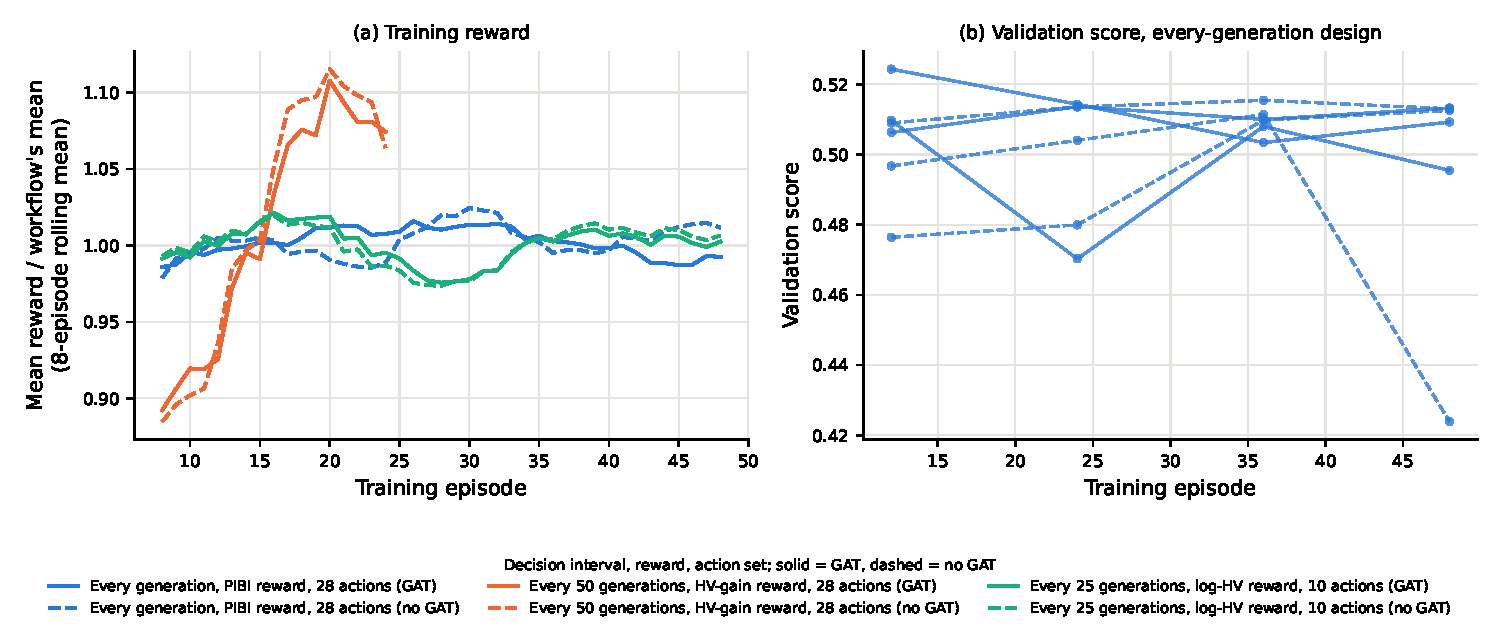
\includegraphics[width=\linewidth]{figures/d1_training.pdf}
\caption{Training of the three learner designs. (a) Reward per episode relative to the workflow's mean, 8-episode
rolling mean over training seeds. (b) Validation score of the per-generation agents.}
\label{fig:training}
\end{figure}

\begin{figure}[!htbp]
\centering
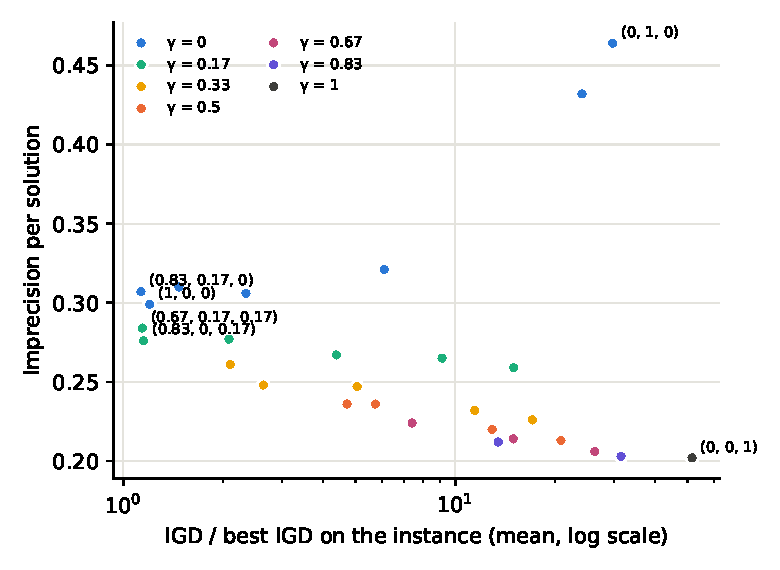
\includegraphics[width=0.6\linewidth]{figures/a3_tradeoff.pdf}
\caption{IGD ratio to the best action against imprecision per solution for the 28 fixed actions on the 36 training
instances. Colours mark the uncertainty weight $\gamma$.}
\label{fig:a3_tradeoff}
\end{figure}

\end{document}
